\chapter{Classifying Meteorological Observations in Radar Image Data}
\label{sec:classifying}

%Might need to have more information on general data handling. 
%One idea: Do some in-class similarity statistics on various classes in meteorology data as well as some toy dataset. 
%Might need to have entire section on toy dataset even.

A question of particular interest is that since most available convolutional bases are trained on photographic images, can the knowledge from the structures, textures, and features they extract be applied to data outside the natural image domain?
These models are trained for 3 input channels, which are usually red (R), green (G), and blue (B), to form the 3-tuple denoted RGB.
In the \textit{reflectivity alone} case, there is a single channel of image data, which is simply the $Z_h$ intensity value.
There is usually, however, color information that is applied to this data via a colormap, which both quantizes the data and assigns color to this data bins. 
This is usually intended as a method to enable ease of visualization for humans, both in real-time analysis as well as when examining prior data.
A common practice to facilitate the human-data-discovery pipeline is to store generated images as \textsc{png} files, or some other image specification.

As such, this method sets up a convenience in data processing, if it can be incorporated into a machine learning pipeline as a direct input, thus saving costly steps involving file I/O, reading specific variables data, and processing into a suitable format. 

This leaves a few specific questions for this work:

\begin{itemize}
	\item Can a deep learning (DL) model learn from and properly classify single channel data?
	\item Can it do so from a colormapped version of the data?
	\item Is there a specific colormapping technique that would yield a more suitable or even optimal mapping ot use as input to a DL model?
\end{itemize}

We designed and present a few experiments, designed to answer these questions.
The first question is one that is key in this dissertation.
Put another way, can low- and mid-level image features be used in weather radar image data to identify and classify precipitation regimes?
This question will be answered over the course of this manuscript.
However, the following two questions need to be addressed as part of this, and will be examined first.

One way that Deep Learning architectures can be thought of working is via extracting image features and analyzing the spatial and pixel-based content, then using these features to discriminate between classes.
RGB tuples are usually the input, which gives 3 independent channels of data for the DL models to analyze.
As such, it seems unlikely that the specific colors used would matter, so long as the space was appropriately trained and modeled, and test images remain consistent with training images.

In order to test this hypothesis, we examine a few colormapped versions of the input MNIST Fashion dataset, which contains $N=60000$ training samples encompassing 10 classes relating to categories of clothing.
The usage of this dataset is to provide a point of comparison for the model accuracy and loss curves generated in this research with benchmark values produced by others in the field.
We will illustrate the design choices regarding constructing and training the end-to-end deep learning model architecture using this dataset prior to implementing it on the desired target dataset of precipitation regimes.
Specifically, we perform the following experiments to answer the following questions:

\begin{itemize}
	\item With many available choices of carefully trained convolutional base models available in the field, which to choose?
		\item Experiment: Compare classification curves of two such models, VGG16 and MobileNetV2, using MNIST-Fashion dataset
	\item Does colormap matter?
		\item Since many available processed weather radar scans involve colormapped data designed for human evaluation, it is important to discover if colormapping intensity values has a deleterious effect on model learning
		\item Experiment: Encode the MNIST-Fashion images in three colormaps, and compare validation accuracy of chosen model on each dataset, which are detailed here:
		\begin{enumerate}
			\item Black \& White: Raw data duplicated in three channels
			\item Viridis: Perceptually uniform, to faithfully match colormap design to data characteristics
			\item NWS Reflectivity: Mapping data to rainbow colormap preferred by the National Weather Service to represent horizontal reflectivity data
		\end{enumerate}
	\item How much can we learn?
		\item Train model on each dataset until maximum learning is achieved in top classifier, then fine tune model to maximize learning on target dataset
\end{itemize}

This chapter first introduces image classification and develops a brief but necessary background in techniques and advances that lead to solving problems of the kind in this work.
There are several conventions regarding nomenclature and formal description of this sets of problems and solutions.
As such, it is critical to establish a convention to be used throughout this document.
Additionally, the open source movement in the research fields has led to an increase in open access publications.
Following along in this spirit, this document will attempt to follow conventions set by respected, oft-cited, open access materials, such as \cite{goodfellow2016}.

\section{Image Classification}
\label{sec:classifying_image}

In order to understand image classification, transfer learning, and the application of these to weather radar images, we must first examine the basics of machine learning, and carry this examination through deep neural networks (DNNs), how these models are developed, and how features can be extracted from images and used to generate predictions, classifications, and ultimately, to generalize to unseen data. 
It is expected that the readers will have had some prior experience in studying machine learning techniques, and as such, the examination here will not be exhaustive. 

It is perhaps important here to specify that image classification is one sub-type of classification problem that is discussed in image-based deep learning literature.
Image classification is to make an inference about the class to which an image belongs in its entirety. 
Contrary to this is object detection, which seeks to find localized objects in a given image.
In object detection, there can be multiple instances of a given object in any image, and it is expected that there are many types of objects that may or may not be present in any image given to the system.


\subsection{Machine Learning Concepts}
\label{ssec:classifying_concepts}

% Training/Testing, Classification/Regression, Supervised
We can define machine learning as a methodology for allowing a program "to learn from an experince $E$ with respect to some class of tasks $T$ and performance measure $P$, if its performance at tasks in $T$, as measured by $P$, improves with experience $E$," as described in an early book \cite{mitchell1997} on the topic. 
This verbalizes and formalizes the experiment space in which machine learning algorithms live.
In this terminology, the task $T$ is what we seek to achieve; in this work, this is always a classification of input data into categories, such as classifying weather radar. 
The experience $E$ is the data that the model learns from, and consists of two types of datasets, referred to as \textit{training} and \textit{validation} data. 
In \textit{supervised learning} problems, the umbrella under which the problems in this work exist, the training and validation datasets have labels corresponding to the correct classification.
These labels are used to teach the model how to classify the data samples presented during the training phase.
Additionally, the validation set is a group of data samples representing a stratified random sample of all samples available in training, and is used to evaluate the model during training to provide information to both the model itself and the researcher.
The performance measure, $P$, is how the predictions of the model are evaluated, which usually takes the form of an \textit{accuracy}, which is computed as the fraction of correctly predicted values to the total number of values.
This is evaluated on a held-out \textit{test} set of data, which is a simulation of unseen data, and is useful as a measure of the model's ability to generalize to heretofore unseen, or potentially new, data.

Many problems in machine learning relate to an experience $E$, or a dataset, where individual samples can be drawn from generating distributions as vectors of some set of features of interest.
In the most classic example of this type of dataset, \cite{fisher1936use} describes a dataset consisting of 3 different types of Iris flowers (i.e, classes), where each individual flower (sample) is described in terms of a set of quantitative characteristics (features).
Many textbooks use this as a well-defined problem- and data-space to introduce these concepts.
We could define a \textit{design matrix} $\textbf{X}$ composed of all data samples in the Iris dataset as $\textbf{X} \in \Re^{150x4}$, as there are 150 samples corresponding to individual flowers, each represented by 4 real-valued quantitative features.

\subsection{Shallow Networks}
\label{ssec:classifying_shallow}

Shallow networks, also referred to as multilayer perceptrons, describe the most basic formulation of neural networks. 
There is a set of inputs, $\mathbf{x}_1$, a set of layers $l$, outputs for each layer $\mathbf{y}_l$, which are functions themselves of weights matrix $\mathbf{W}_l$, the inputs, and biases $\mathbf{b}_l$. 

Neural networks borrow nomenclature from the field of neurology, and as such, the smallest "cell" in a neural network is called a "neuron." 
In computing, these neurons are made up of connections to the outputs from the previous layer, compute a linear combination on these inputs with a set of individual weights and biases, and the output generates the values for the next set of layers.

The idea behind neural networks is essentially to set up a function that has the ability to "learn" a dataset's inherent class distributions by looking at the data, passing it through this model architecture, computing the combinations of input variable values, propagating through the layers, and making some prediction at the output layer. 
In classification problems, this output prediction is of class membership, hence the term "classification." 
Neural networks can also be used in regression problems, but that usage is out of scope for this work.

In the simplest example of a multilayer perceptron, there is a layer of inputs, an output, and one neuron.
This case is identical to \textit{linear regression}, and can be represented as

\begin{equation}
y = \textbf{w}^T\textbf{x} + b
\end{equation}

where $\textbf{w}$ is a vector of weights, $\textbf{x}$ is the vector of inputs, and $b$ is a bias term.

In order for this model to learn, there must be a way to evaluate its predictions. 
There may be many ways to evaluate predictions, some optimal given a particular data set or end goal, but one common method is to the \textit{mean squared error}. 
The mean squared error in this case is given by

\begin{equation}
\textrm{MSE}_{test} = \frac{1}{m}\sum_{i=1}^{m}\left(\hat{\textbf{y}}^{test}-\textbf{y}^{test}\right)^2
\end{equation}

where $m$ is the number of data samples in the test set, $\hat{\textbf{y}}^{test}$ is the labels predicted for the test set, and $\textbf{y}^{test}$ is the true labels.
The error above will be minimized when all predicted labels match the true labels.
The goal in training any machine learning model is in altering the weights vector $\textbf{w}$ (or matrix $\textbf{W}$) and bias $b$ such that the amount of correctly predicted labels increases.
This is generally achieved by employing a \textit{loss} function to compute the error, or loss, between predicted values and true labels.
The loss function is another way to evaluate model performance $P$, and choice of loss function is important, determined by both the data space, the type of machine learning algorithm, and the desired output.

Since the objective in training is to minimize the loss, we can compute the \textit{gradient}, the partial derivative of the objective function at every layer with respect to outputs, and minimize that. 
More formally, we allow our model to experience the training data set and its labels, ($\textbf{X}^{(train)}$, $\textbf{y}^{train}$). 
In the simple case of linear regression, we seek to minimize the gradient on the training set, 

\begin{equation}
\nabla_\textbf{w}\mathrm{MSE}_{(train)} = 0
\end{equation}

Substituting,

\begin{equation}
\nabla_\textbf{w} \left| \left| \hat{\textbf{y}}^{(train)} - \textbf{y}^{(train)} \right| \right|_2^2 = 0
\end{equation}

from which the optimal set of weights can be computed following \cite{goodfellow2016} as

\begin{equation}
\textbf{w} = \left( \textbf{X}^{(train)^T} \textbf{X}^{(train)} \right)^{-1} \textbf{X}^{(train)^T} \textbf{y}^{(train)}
\end{equation}

While this function has an optimal set of weights that can be determined analytically, it is unfortunately too limited to be of much use in more complicated problems, such as those involving modeling non-linear class distributions, as well as "deeper" models, or those with image inputs. 
To search for solutions in these problem spaces, we must employ deep feedforward network models, a class of models in the field of deep learning.

\subsection{Deep Feedforward Networks}
% This is where to discuss nonlinear learning, depth of networks, and gradient-based learning via backpropagation

Deep learning implies \textit{depth}, a concept that is suitable and relevant in deep feedforward networks, a class to which the deep convolutional neural networks utilized in this work belong. 
In this context, depth corresponds to many layers of many neurons each, generating many, many more connections than in shallow network architectures.

The goal of a deep learning model is to satisfactorily approximate some function $f(\cdot)$, that maps inputs $\textbf{x}$ to output categories $\textbf{y}$, with some set of parameters $\bm{\theta}$.
The general function can then be written as

\begin{equation}
\textbf{y} = f(\textbf{x};\bm{\theta})
\end{equation}

As above, we follow the standards and nomenclature presented in \cite{goodfellow2016}, etc, in this work.

The name 'feedforward' comes from two aspects: first, that information flows from inputs to outputs \textit{forward} through the model; and, values propagate from input to output without any \textit{feedback} connections to previous layers, as is sometimes used in memory-based models like recurrent neural networks\cite{graves2009novel}, or models that take inspiration from such connections, such as ResNet\cite{he2016deep}.

There can be many intermediate functions, or \textit{layers}, between input and output, connected via a chain of functions, such as

\begin{equation}
f(\textbf{x}) = f^{(1)}(f^{(2)}(f^{(3)}(\textbf{x})))
\end{equation}

where the superscript $^{(l)}$ denotes the function at layer $l$. The term "deep" learning in part comes from the usage of many of these such layers, or more generally,

\begin{equation}
f(\textbf{x}) = f^{(1)}(f^{(2)}(\cdots f^{(l)}( \cdots f^{(d)}(\textbf{x}))))
\end{equation}

for $d$ layers.

There is one more limitation in shallow models to overcome prior to designing a deep architecture capable of modeling general functions: nonlinearity.
One way to account for this is to apply a nonlinear mapping on the inputs at each layer $\phi$ such as $\phi(\textbf{x})$
This can be managed in multiple ways: specifying a general nonlinear function for the inputs, leading to a class of problems including support vector machines \cite{cortes1995support}; manually designing the function, analogous to many empirical and theoretical strategies in many fields involving decades of work; and learning the mapping, as is done in deep learning.

Formally, we can express this as

\begin{equation}
y=F(\textbf{x}; \bm{\theta},\textbf{w}) = \phi(\textbf{x};\bm{\theta})^T\textbf{w}
\end{equation}

with parameters $\bm{\theta}$ to be drawn from a class of nonlinear functions, and weights $\textbf{w}$ to be learned to map the inputs to the output type of interest.

Generally, the weights vector $w$ is initialized to random small values, training samples are input to the system, and the loss is calculated between predicted and true labels for the output.

This phase is often referred to as \textit{forward propagation}.
It is worth noting that recent works have shown \cite{glorot2010understanding} \cite{he2015delving} that more carefully initialized weights can lead to more stable properties in deep learning models, discussed later in this work.

In the next phase of training, \textit{backpropagation}, the gradient of the loss function is calculated.
The loss function, or \textit{cost} function, needs to be minimized, which in turn improves the understanding by the model of the dataset.
Computing an analytical solution of a single neuron, feedforward neural network, as above, is not infeasible.
Doing so for shallow neural networks, featuring a relatively small number of parameters to optimize may be reasonable in some cases, but doing so in a deep neural network, where the number of parameters may extend into the tens of millions is not only intractable but likely impossible.
However, if the specified loss function is differentiable, we can use its gradient calculated with respect to the parameters as a way to seek local minima in these high-dimensional spaces.
Doing this allows the network to learn by adjusting its weights, backpropagating changes informed by moving in the opposite direction of the gradient, which seeks to minimize the loss and increase learning.

% more considerations to include: need lots of data, stochastic gradient descent, fine tuning.
% this last will be referred to in the benchmarking section below
\subsection{Layers and Activations}
\label{ssec:classifying_layers}

Training a neural network is a nontrivial task, even when the details of stochastic gradient descent and basic connection types have been worked out.
Specifically, we examine a subset of the available layers and activation functions, focusing those that will be used in this research in the top classifier.

There are two layers called \textit{batch normalization} layers, and these are used to shorten training times and make it less likely that either vanishing or exploding gradients are encountered.
These two issues form one of the core challenges in training a deep neural network, and are often the result of poorly initialized weight vectors $\textbf{w}$ or as a consequence of the many layers present in a deep neural network.
One way to counter this is to include normalization steps, where weights in each batch normalize inputs to these specific layers.
This was introduced in \cite{ioffe2015batch} to reduce this internal covariate shift, and uses batch statistics in the following algorithm from their paper:

\begin{itemize}
	\item Input: values of $x$ in a particular batch, given by $B={x_{1\dots m}}$ with parameters to be learned, $\gamma, \beta$
	\item Output: ${y_i=BN_{\gamma,\beta}(x_i)}$
	\begin{enumerate}
		\item Compute mini-batch mean: $\mu_\beta = \frac{1}{m}\sum_{i=1}^{m}x_i$
		\item Compute mini-batch variance: $\sigma_\beta^2 = \frac{1}{m}\sum_{i=1}^{m}(x_i-\mu_beta)^2$
		\item Normalize inputs: $\hat{x}_i = \frac{x_i-\mu_\beta}{\sqrt{\sigma_\beta^2+\epsilon}}$
		\item Scale and shift: $y_i = \gamma\hat{x}_i + \beta \equiv BN_{\gamma,\beta}(x_i)$
	\end{enumerate}
\end{itemize} 

where $x_i$ is and input, $B$ is the set of inputs in the training batch, and $\epsilon$ is a small non-zero weight that ensures no division by zero is possible.

This is ultimately a relatively straightforward calculation, but by normalizing inputs at late stages, we saw a marked increase in the network's ability to learn.
At the stage this is employed, the inputs themselves are the many feature tensors produced by the convolutional base, which are in turn the resulting feature maps from the image data, which itself could be drastically different from image to image.
It is believed that the batch normalization defuses some of the issues with these disparate inputs.

In order to generalize to nonlinear functions, we must introduce a nonlinear mapping $\sigma(\cdot)$ somewhere in the network.
It is most often applied to each neuron, such that $\hat{y}_i = \sigma\left(\textbf{x}\textbf{w} + b\right)$. 
There are many choices for this function, though the most common is the rectified linear unit, or ReLU.
This was designed in part as an analogy to activations in the brain, though the ReLU can take on more potential values.
It is given by

\begin{equation}
\sigma(\cdot) = \mathrm{max}(0,x)
\end{equation}

There are many variations on this, including noisy ReLUs, leaky ReLUs, and Parametric ReLUs, though these are not employed in this research and will not be discussed.

Finally, in training it can be good to randomly zero out neurons in order to mitigate effects of overfitting.
This is based on the assumption that if a network is unable to "count on" any neuron or set of neurons during training, redundancy will be built into the network, and also generalizability, since no set of neurons can learn specific features in specific images.

The rate of dropout varies, and studies point out that more or less may be useful given the application and other layers. 
The authors of the batch normalization paper suggested that dropout could itself be dropped out of networks in many cases when batch normalization was employed, though it was found through experimentation that a dropout rate of 0.33, or 33\%, worked well in this research.

\section{Benchmarking Deep Learning Methods with MNIST-Fashion}
\label{sec:classifying_benchmark}
% Talk about the effort to standardize this on a dataset well-studied and well-understood
% specifically, the MNIST-Fashion

Given the complexity of the task at hand and the need for an experiment framework that can be compared to other efforts in the field, it may be relevant and useful to use a known dataset to benchmark the algorithms we develop in this work.
As such, this section details the effort to standardize the experiments on a well-studied and well-understood dataset.

\subsection{Dataset}
\label{ssec:classifying_dataset}
Historically, the MNIST dataset\cite{lecun1998gradient} has been employed as a method for ensuring that results from research in various computer vision tasks are valid and comparable to a well-understood baseline.
Unfortunately, the MNIST dataset has recently been considered to be overused\cite{xiao2017fashion}, leading to many models that are excellent at classifying the handwritten digits dataset, but not optimally generalizable to more complex tasks arising from images that include more features and more overlap.
It has also been pointed out that MNIST-trained algorithms do not find general representations in computing feature maps, leading some researchers to believe that models often simply memorize the training data to generate the high levels of accuracy often observed in state-of-the-art architectures.

As a result, we have chosen to forego usage of the MNIST dataset in favor of a more complicated dataset called MNIST-Fashion \cite{xiao2017online}.
This dataset consists of 70,000 images representing 10 classes of items of clothing.
The images are square and equally sized ${28 x 28}$, single-channel intensities on black backgrounds.
These design choices mirror those in the original MNIST dataset, which is based on the desire for a drop-in improved replacement for the oft-used digit recognition database.
Some example images in each class are shown in Figure \ref{fig:classifying_fashion-mnist}.

This research draws upon insights provided in the field of transfer learning, and as such, uses a trained model as its \textit{convolutional base} layer.
The goal of this layer is to utilize general low- and mid-level image features present in many images, and train a \textit{top model} classifier initialized from random weights to learn to classify the \textit{target} task.
It is specified that as a rule of thumb, the target task should not be very different from the source task that the model was trained upon\cite{yosinski2014transferable}.
Throughout this work, however, the goal is to classify weather radar images, which are quite different from the natural images that most available models were trained upon.
Another benefit of benchmarking on the MNIST-Fashion dataset, though, is that it too represents a set of images that differs from the ImageNet dataset \cite{imagenet_cvpr09}, which is what the convolutional base models were trained upon, a dataset containing more than 14 million natural images representing 20,000 classes.
The MNIST-Fashion images are natural images, but they also are similar to the single-variable weather radar data as well, in that they contain information in only one channel.
It is expected that this dataset is thus similar to both source and target tasks, whereas the two are themselves quite different.

\begin{figure}[h]
	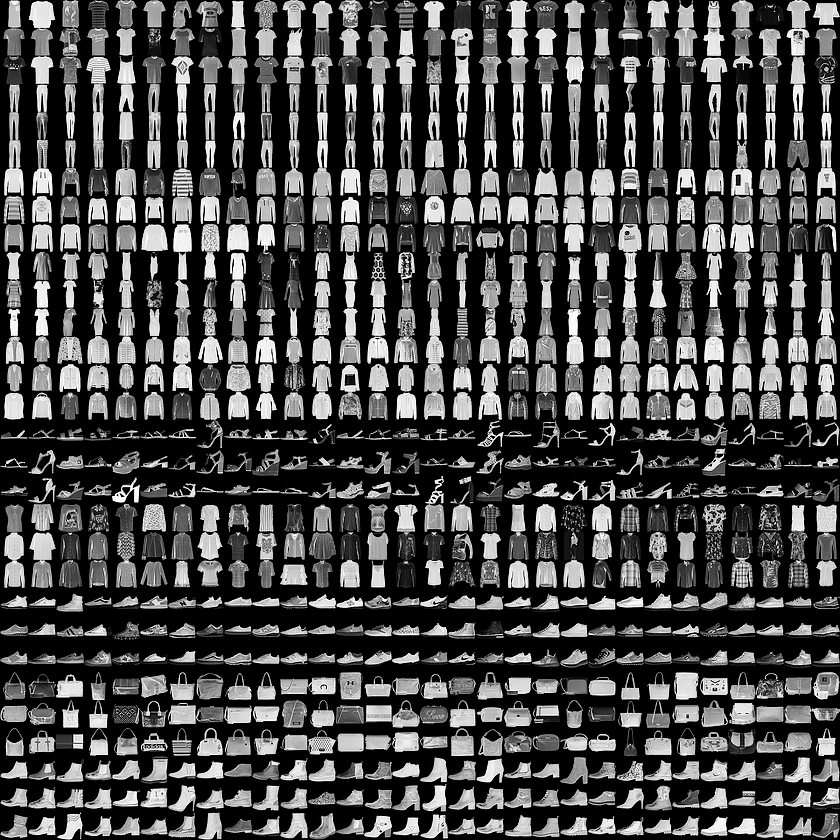
\includegraphics[width=\textwidth]{thesis_code/fashion-mnist-sprite.png}
	\caption{Examples from each class in the MNIST-Fashion Dataset. Each class is represented by three rows in the figure.}
	\label{fig:classifying_fashion-mnist}
\end{figure}

\subsection{Selecting a Convolutional Base}
\label{ssec:classifying_selectingbase}
Before turning to single-channel weather radar data in Section \ref{sec:classifying_zhcasa}, we must design an end-to-end model capable of matching or exceeding MNIST-Fashion benchmark error rates using a convolutional base trained initially on the ImageNet dataset.
There are several readily available models from which to choose \cite{chollet2015keras}.
It is assumed that in the well-trained case, a larger model corresponds to better generalization to unseen data, as there is more room within the architecture to model more features relevant to classification.
Meanwhile, smaller models may be have shorter training time necessitating less compute power, at the cost of generalization power.

To test this, we designed an experiment involving one well-known deep learning architecture from each category.
The VGG16 \cite{simonyan2014very} architecture represents a large model, at 528 MB, while MobileNet version 2 (MobileNetV2) \cite{sandler2018mobilenetv2} is much smaller, using 14 MB memory.
See Table \ref{table:classifying_conv_bases} for technical specifications of each model.

\begin{table}
\begin{tabular}{l r r}
	Model & Size & Parameters \\
	\hline
	VGG16 & 528 MB & 138,357,544 \\
	MobileNetV2 & 14 MB & 3,538,984 \\
\end{tabular}
\caption{Some relevant technical characteristics of two deep learning architectures}
\label{table:classifying_conv_bases}
\end{table}

Each convolutional base requires data to be formatted in a specific manner: input images must be normalized on the interval $[0,1]$; they must be a specific size, $[96 x 96]$; and they must contain three channels, since the convolutional bases were trained on three-channel RGB natural images.
In order to conform to these requirements, all training and testing images were generated from the dataset by a combination of upscaling the resolution and duplicating the single channel data to three channels, effectively retaining the black \& white input nature of the raw images.
At training and validation time, images were scaled from $[0,255]$ to $[0,1]$.
During training, data augmentation was utilized in an effort to "fake out" more data, as well as to attempt to make the network more generalizable to translations and scaling in the images.
Specifically, input images were centered and normalized, as well as randomly horizontally flipped.

We demonstrate the usage of each convolutional base using the same top model.
The top model uses as input the features extracted in each convolutional base, and learns to classify the target dataset using those features while training its own set of parameters.
Through theoretical and empirical processes, a relatively small top model consisting of 6 layers was chosen.
This set of layers includes batch normalization, global average pooling, dropout, dense connections, and its final output layer is a softmax classification layer.
An example diagram illustrating a top-down view of the end-to-end classifier is shown in Figure \ref{fig:classifying_architecture}.
During training, the weights in the convolutional base model are held constant, to preserve the findings from training on the ImageNet dataset and to provide the top model consistent inputs while it learns.
No fine-tuning was employed in this test.
Results of training can be found in Figure \ref{fig:classifying_conv_bases}.

\begin{figure}[ht]
	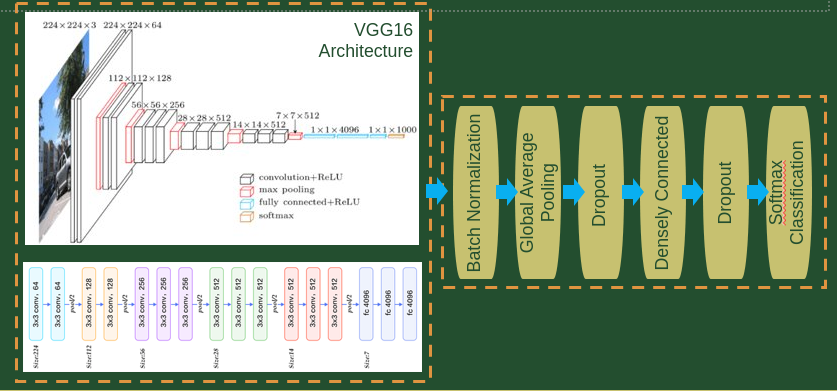
\includegraphics[width=\textwidth]{./thesis_code/vgg16_top_model.png}
	\caption{End-to-end deep learning architecture, with VGG16 convolutional base and bespoke top model.}
	\label{fig:classifying_architecture}
\end{figure}

\begin{figure}[ht]
	\centering
	\begin{subfigure}[b]{\textwidth}
		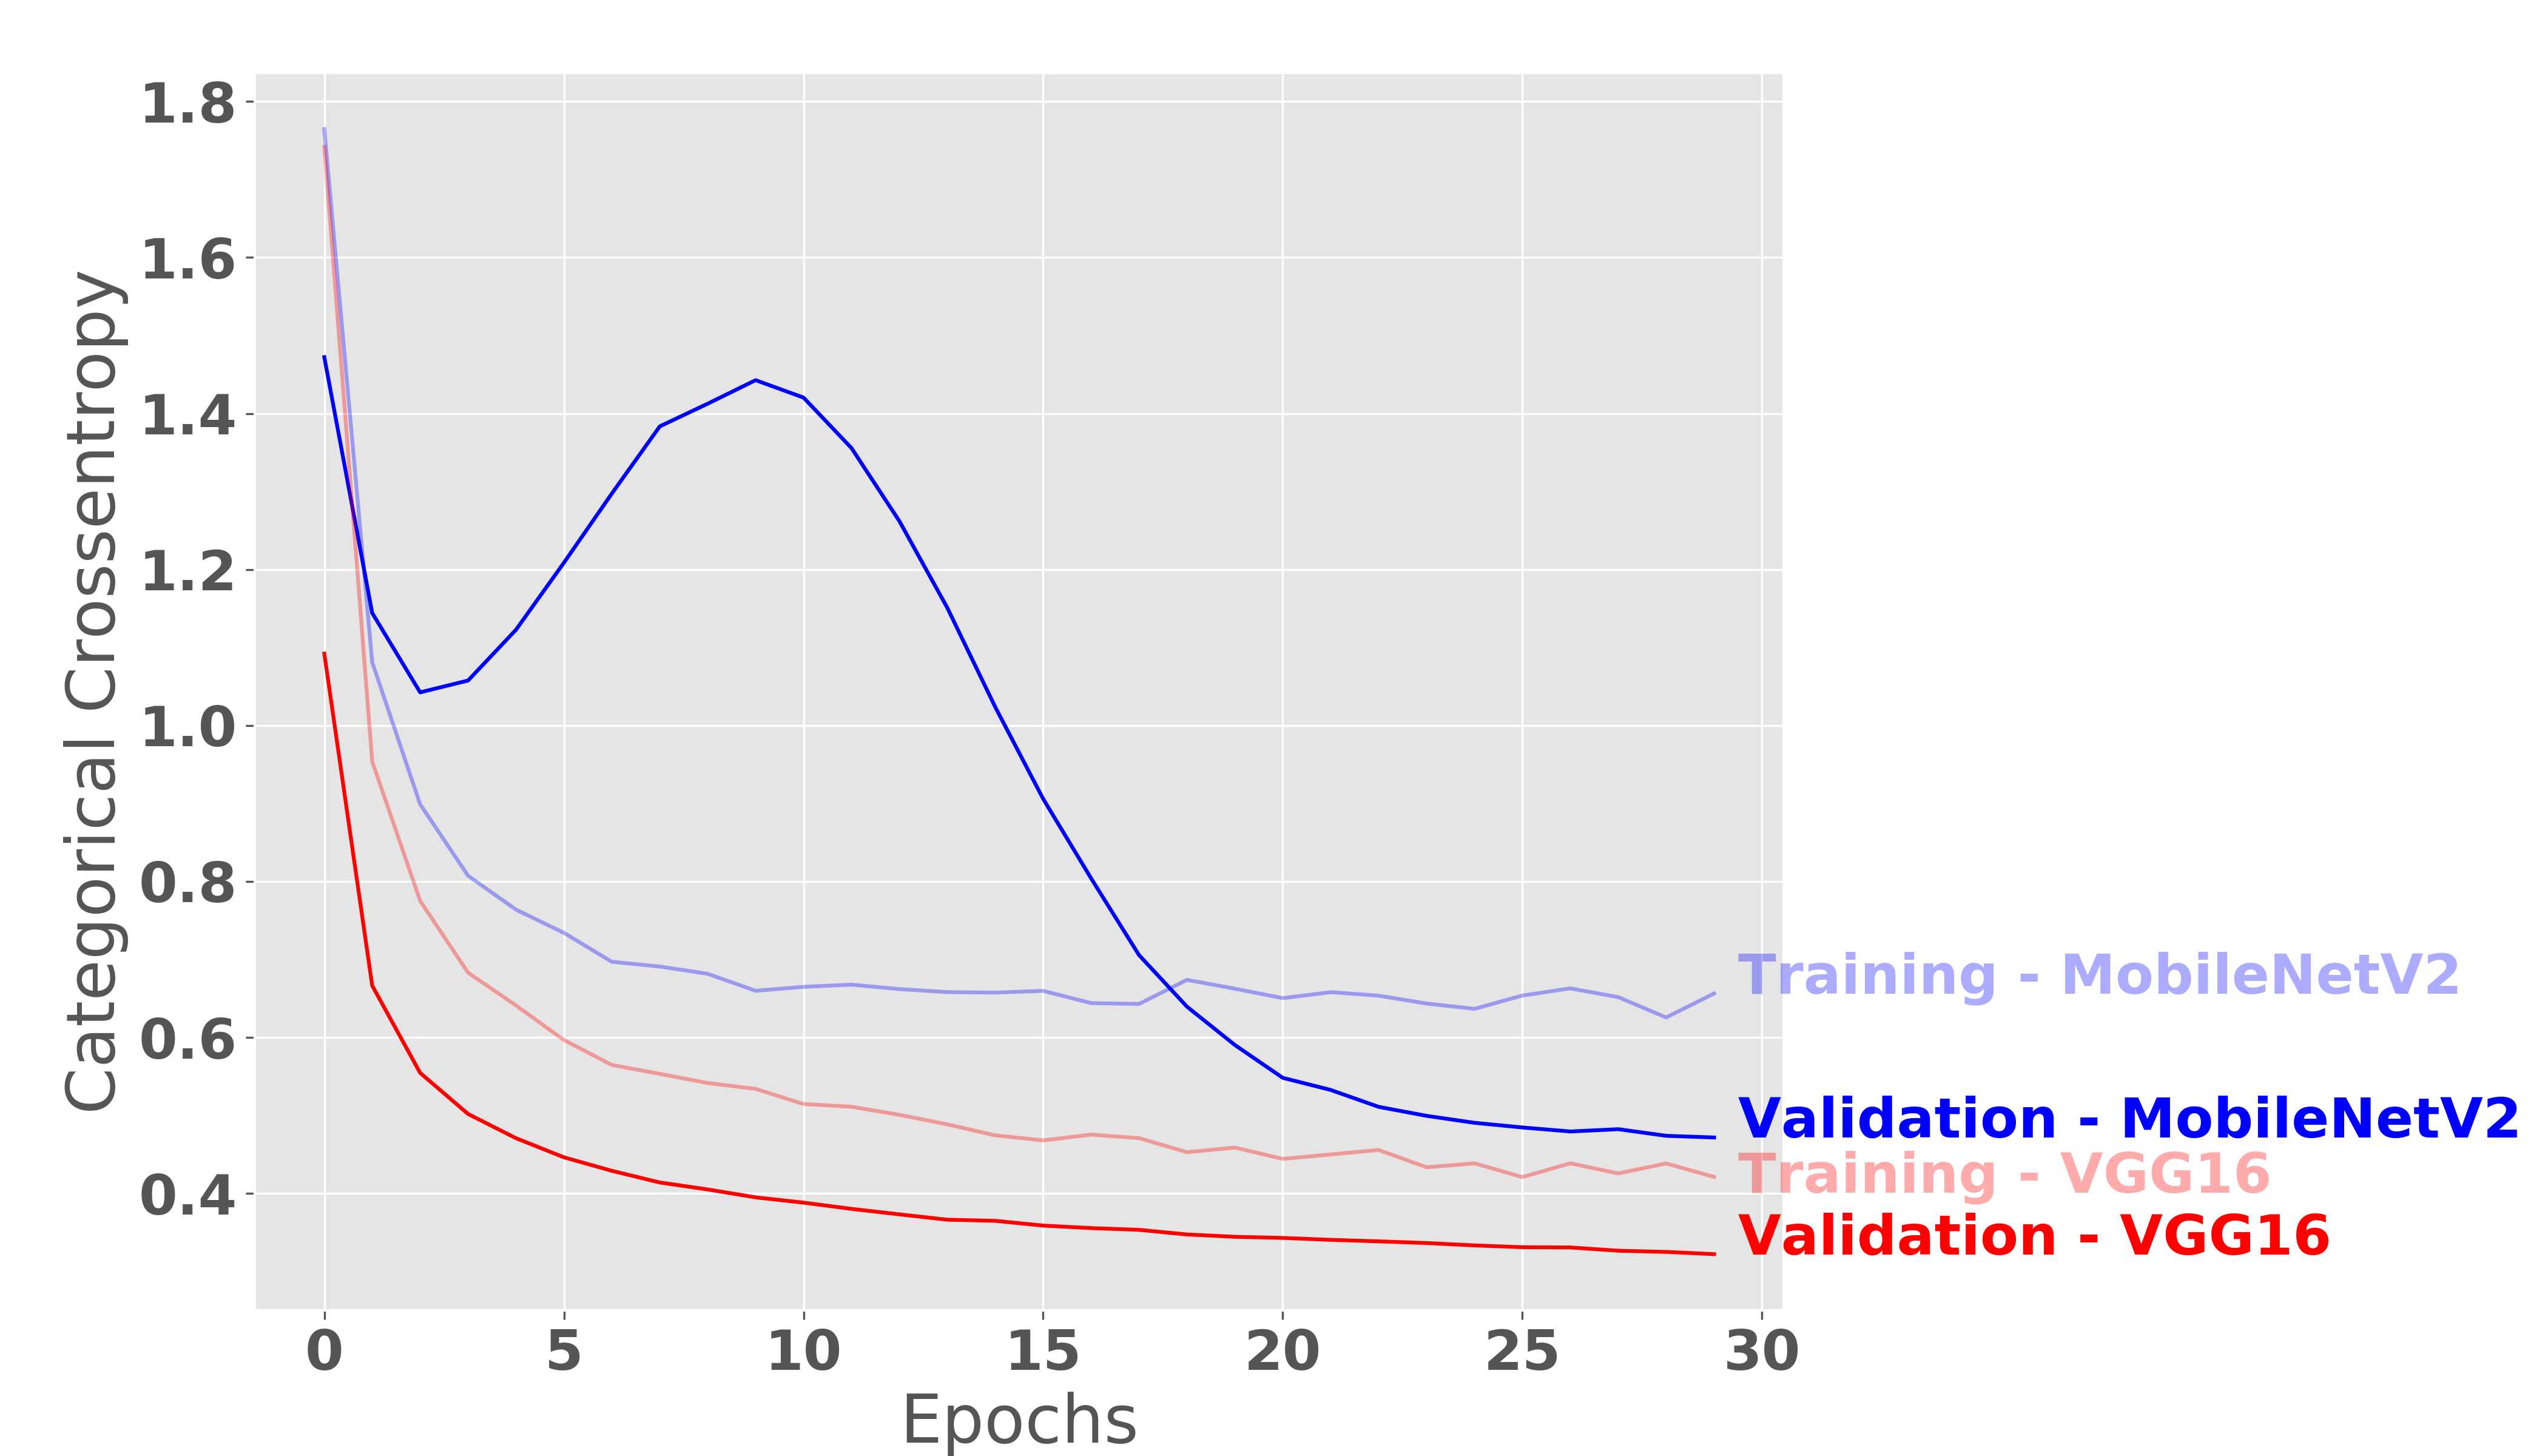
\includegraphics[width=\textwidth]{./thesis_code/plots/train-val-loss_two-nets_three-channels-duplicated.png}
		\caption{Loss}
		\label{fig:classifying_conv_bases_loss}
	\end{subfigure}
	\begin{subfigure}[b]{\textwidth}
		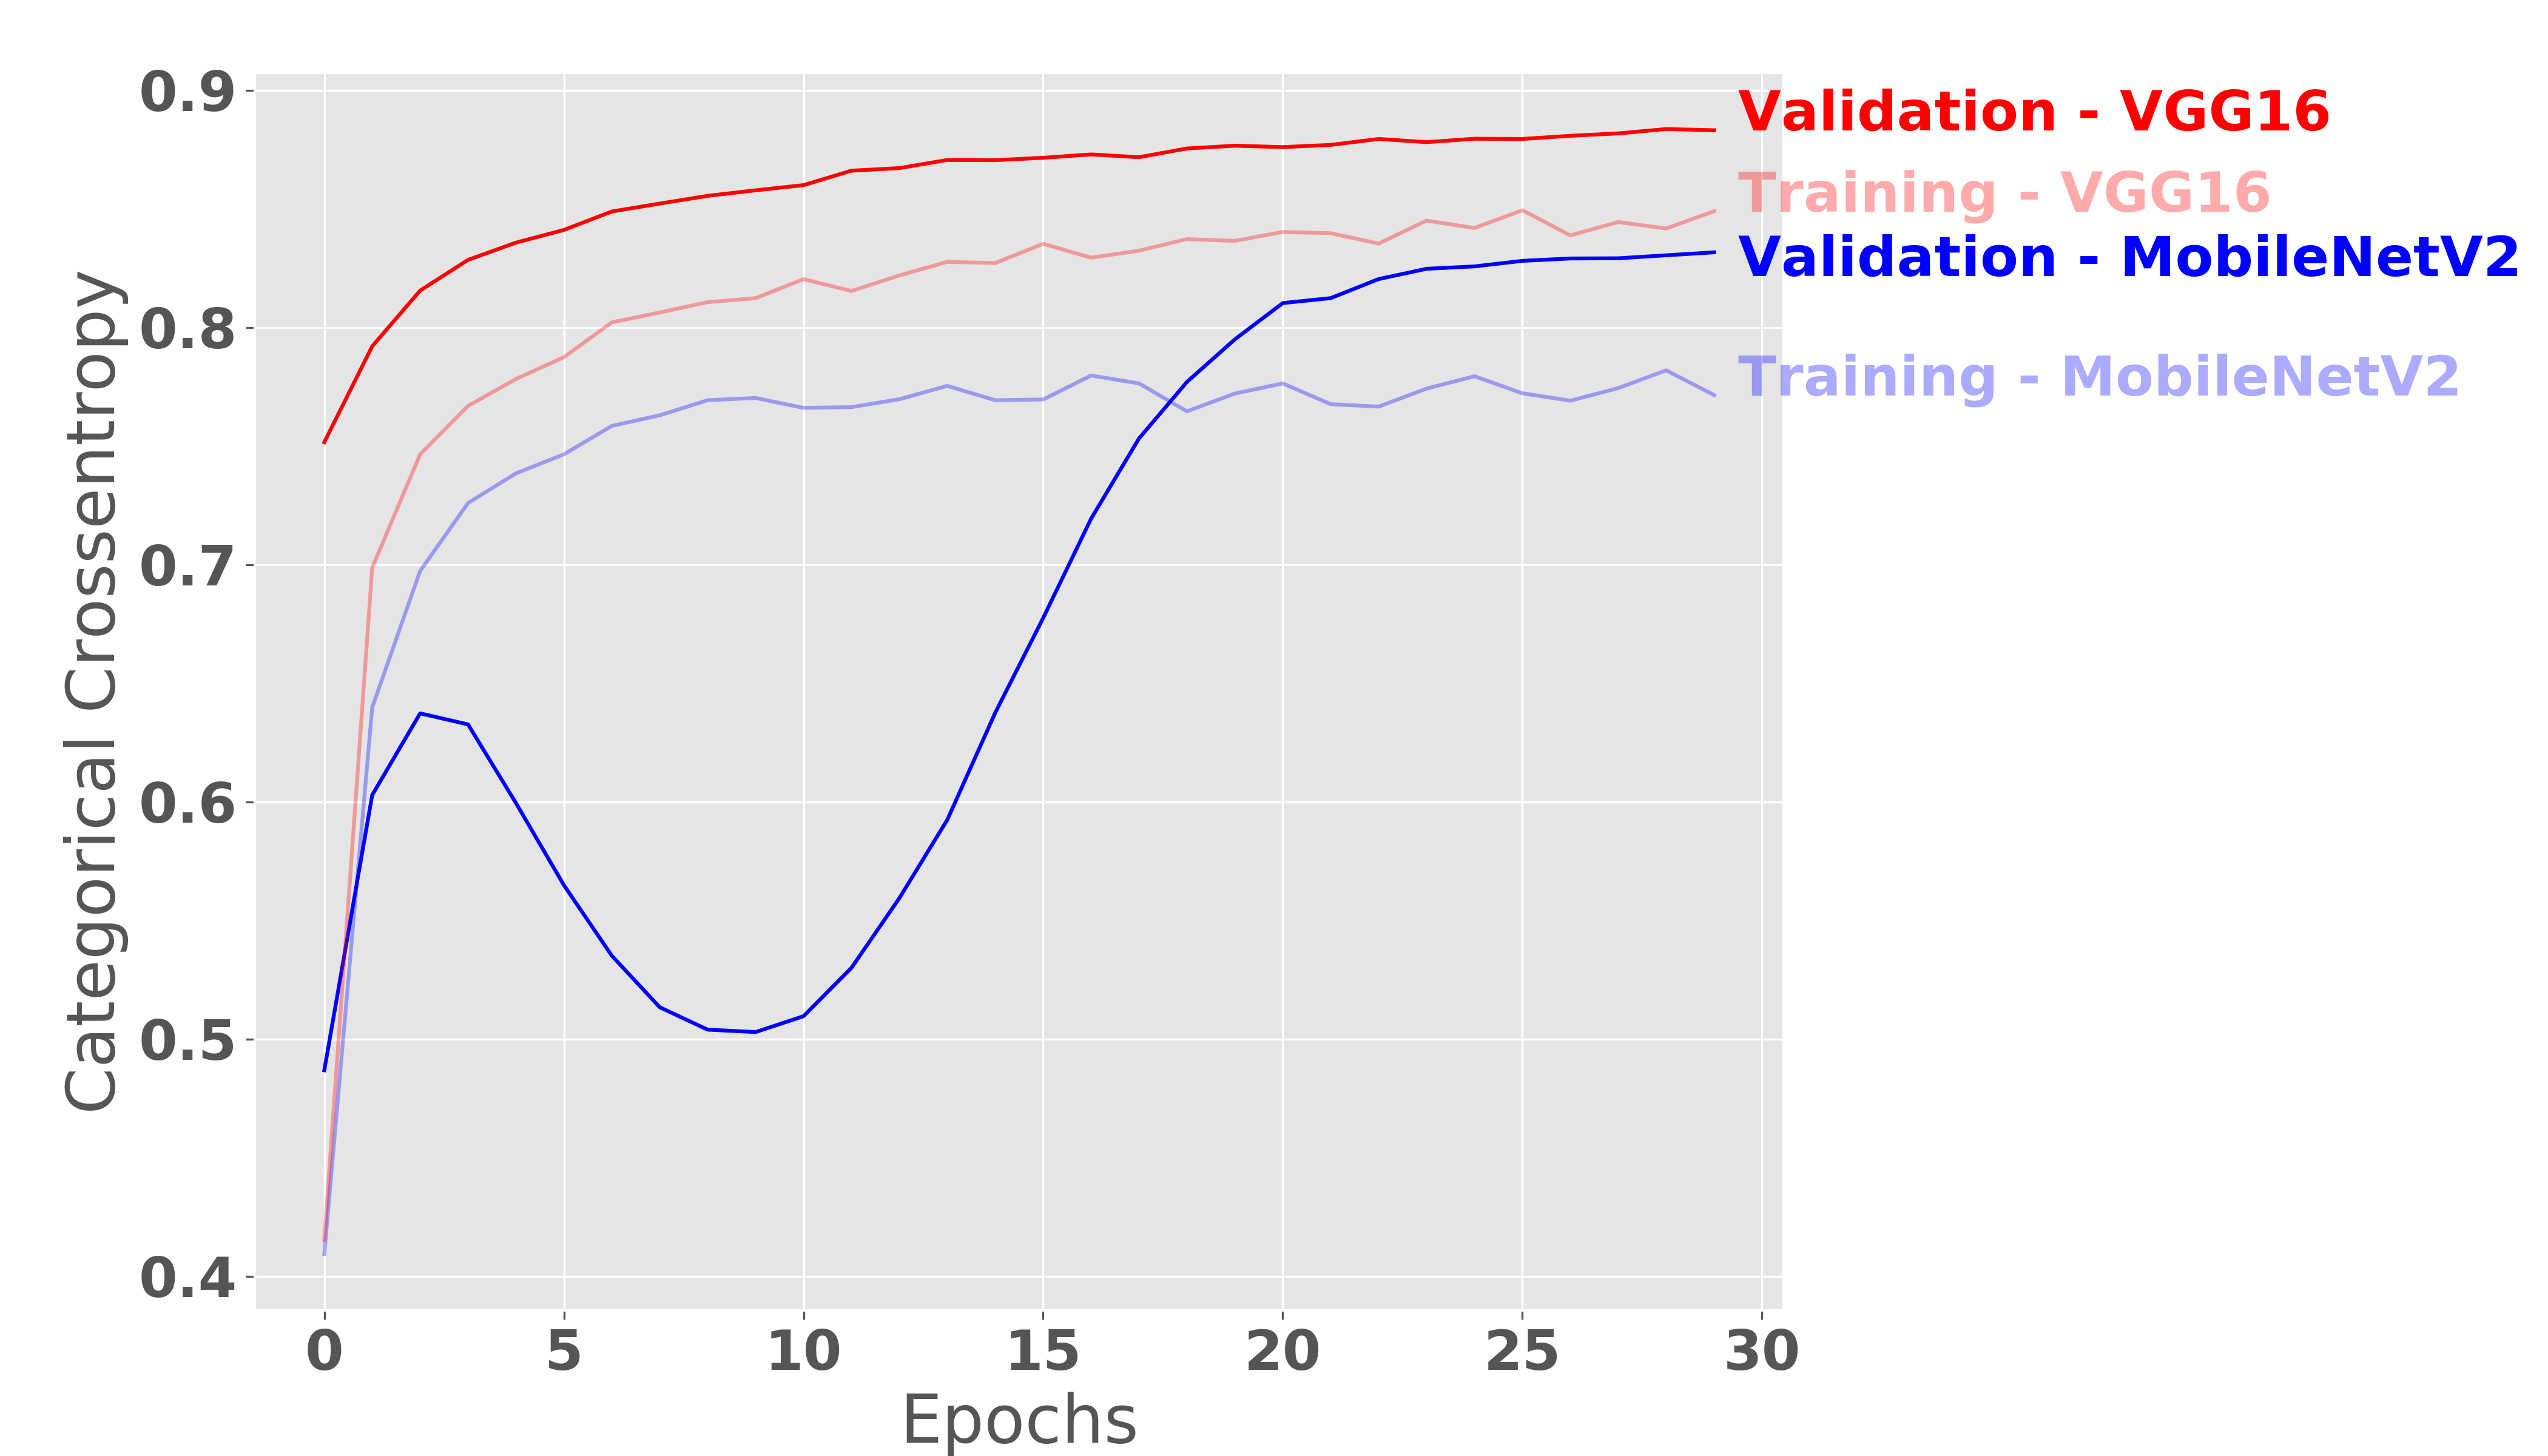
\includegraphics[width=\textwidth]{./thesis_code/plots/train-val-acc_two-nets_three-channels-duplicated.png}
		\caption{Accuracy}
		\label{fig:classifying_conv_bases_accuracy}
	\end{subfigure}
	\caption{VGG16 and MobileNetV2 training and validation characteristics during training on MNIST-Fashion dataset.}
	\label{fig:classifying_conv_bases}
\end{figure}

The results are interesting. Training was limited to 30 epochs, and while the loss had not completely leveled off at epoch 30, the results indicate that on the validation set, the VGG16-based model had a lower loss than the MobileNetV2 version.
This is in line with expectation, as the MobileNetV2 is intended as a valuable tool in performing classification on systems of limited compute power, but such limitations inhibit its ability to approach the accuracy found in larger models.
As such, the analysis in this work will focus on utilizing VGG16 as the convolutional base in classifying weather radar data.

Additionally, there is a region of interest with respect to the training characteristics of the MobileNetV2 model, where validation loss increases while training loss decreases.
It is unclear why this occurs in early epochs, though it is likely due to early overfitting when the smaller model perhaps memorizes the dataset.
Interestingly, this phase ends around epoch 10, where validation loss begins to decrease again and ultimately crosses the training loss.

That validation loss is lower than training loss at the end of training may seem to be counterintuitive, since the validation data is unseen when training batches.
However, this is not an uncommon result when using data augmentation in training.
The validation images are drawn from a held-out portion of the training dataset, but during validation, no data augmentation techniques are applied.
Thus, the model can perform better on validation data than the augmented training data, even while said augmentation assists in learning more generalized filters for the images.

Finally, we will see that validation accuracy, when using VGG16 as the convolutional base, can be increased.
Meanwhile, test set accuracy will match current available benchmarks, but in order to achieve this result, the entirety of the convolutional base will need to be made trainable, and many more epochs of training must occur.

\subsection{Does Colormap Matter?}
\label{ssec:classifying_colormap}
% Discussing importance of colormap in informing classifications, if there is any.
% Three tested: Black & White (3 channels duplicated), Viridis (perceptually uniform), NWS Reflectivity (segmented colormap to match weather radar)

Many weather radar variables, such as horizontal reflectivity $Z_h$, are intensity values.
In other words, there is some range of acceptable values from a minimum to a maximum value, and higher values indicate more intense or higher returns than lower values.
This is somewhat analogous to the type of data in the images in the raw MNIST-Fashion dataset, and as such, similar processing can be applied to the latter dataset to model the former.

Specifically of interest is the type of colormap used to visualize the data.
Weather radar data variables, when plotted as images, usually are represented by a mapping from their raw data space to a color space.
This mapping usually has some forethough behind it as well: radial velocity data, which ranges from a negative to positive Nyquist velocity of scatterers, centered about zero, is typically plotted using a diverging colormap; meanwhile, horizontal reflectivity, where higher values indicate larger and more intense precipitation, is plotted with a segmented colormap where "warmer" colors (i.e, red, orange, purple, white) identify higher returns than color colors (i.e, blue, green, etc).
When such a colormap is applied to data, the values are essentially quantized according to pre-determined bins.
Since $Z_h$ is in dB and since each increase in dB corresponds to an order of magnitude increase in power return of scatterers, these bins are usually kept to a small width; often, 4 dB width to a color, or perhaps "category," of reflectivity returns.
This is designed to inform human viewers as to the contents of the data and the type of scan, but encodes a large amount of potential values and cases in each bin.
Furthermore, such quantization represents a downsampling, so that images of weather radar data have less information than is present in the raw data.
Finally, textures present from this colormapping process in the processed images may represent artificial bounds, relatively arbitrary distinctions leveed upon continuous data.

The above factors raise concern in using pre-generated weather radar data as inputs to a classification model.
As data discovery is a fundamental goal of this research, and as many radar data servers continue to produce colormapped data of this type, it is imperative to discover if such operations impact the classification ability of a deep learning model.
We designed an experiment where the MNIST-Fashion data was colormapped according to three categories to test this:

\begin{enumerate}
	\item Pure Intensity (No colormapping): This is equivalent to the data that was used as input for the above experiment in determining the convolutional base to use
	\item Perceptually Uniform Intensity (Viridis): There has been growing interest\cite{kovesi2015good} in utilizing colormaps designed to appear continuous for human viewers in faithfully representing continuous data, as changes in color appearance can more accurately represent the changes in numerical data. 
	The viridis colormap can be found in many analysis packages in many languages (python\footnote{\url{https://matplotlib.org/gallery/color/colormap_reference.html}}, 
	MATLAB\footnote{\url{https://www.mathworks.com/help/matlab/ref/colormap.html}, listed as 'parula'}, 
	R\footnote{\url{https://cran.r-project.org/web/packages/viridis/index.html}}) and is chosen to represent this class of colormaps.
	\item Segmented Colormap (NWS Reflectivity): The National Weather Service uses a consistent colormap for reflectivity data, similar to the above, where warmer colors indicate higher returns, and cooler colors represent lower return values. 
	This is available in many analysis packages, but this research utilized the Py-ART package\cite{helmus2016python} 'NWSRef'\footnote{\url{http://arm-doe.github.io/pyart/dev/dev_reference/graph.html?highlight=nwsref}} colormap for this experiment.
\end{enumerate}

Refer to Figure \ref{fig:classifying_mnist-fashion_colormaps} for example images from three image classes, represented by each of the colormaps in this experiment.

\begin{figure}[ht]
	\centering
	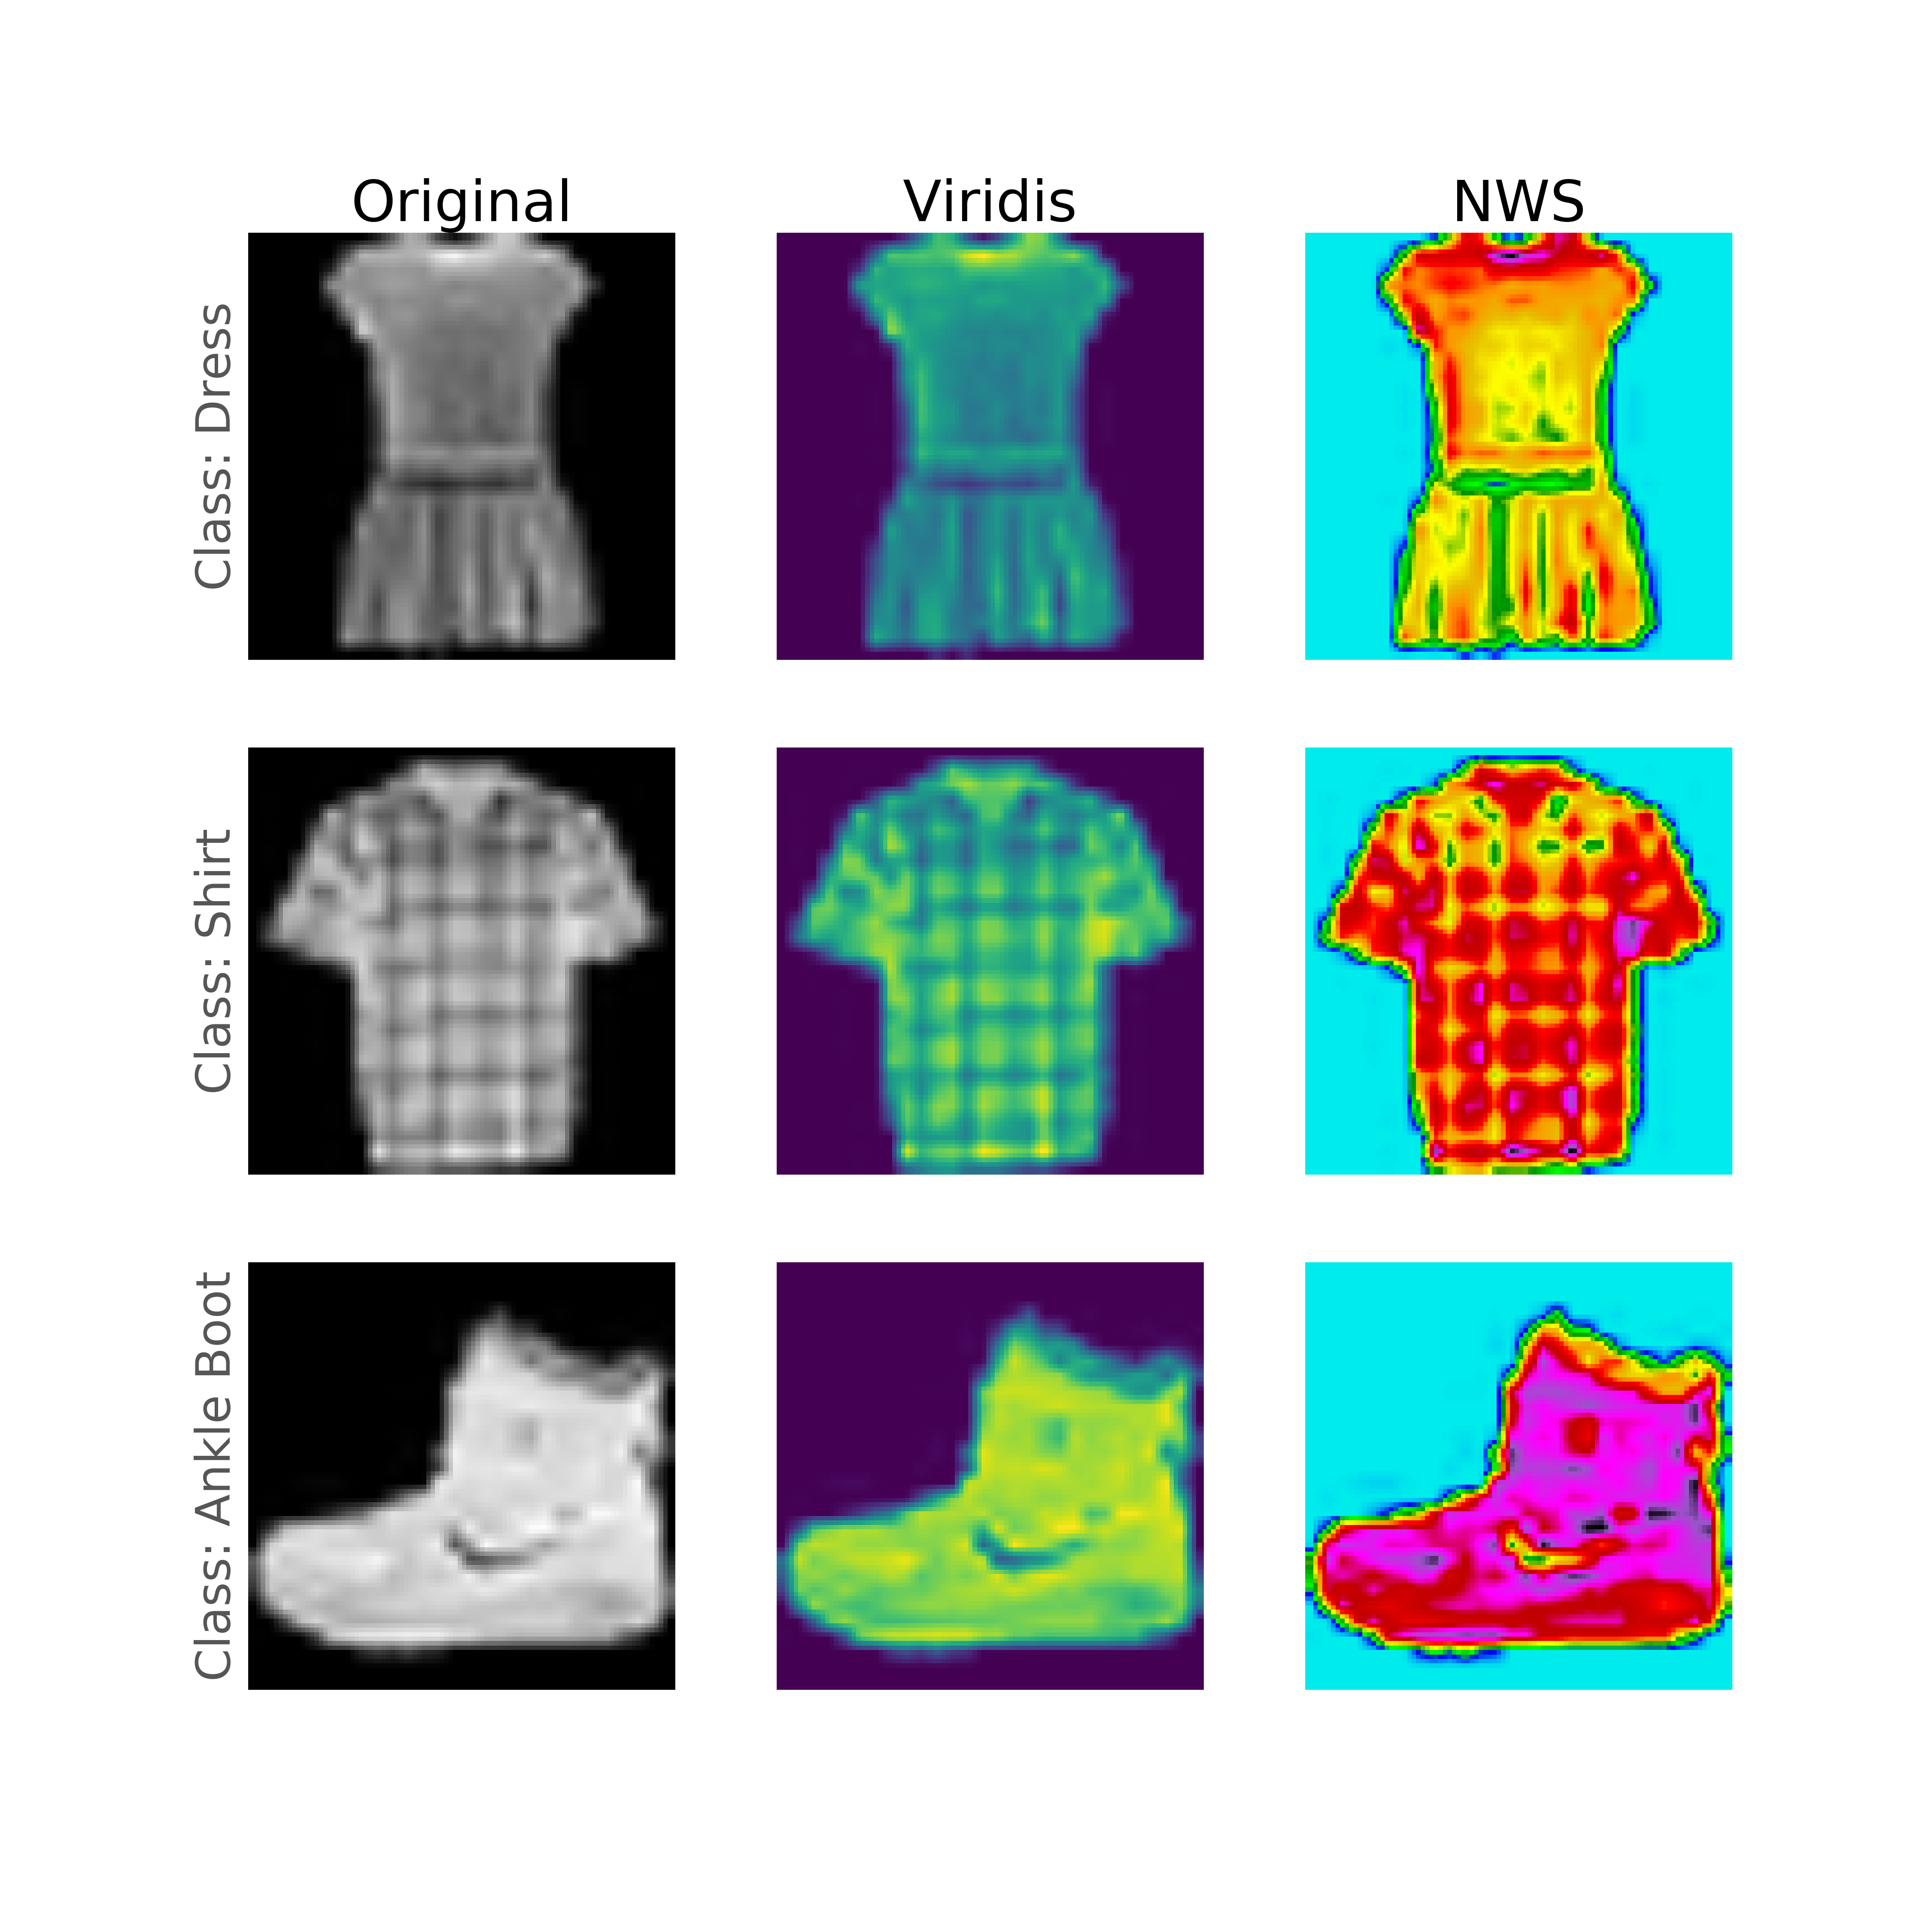
\includegraphics[width=\textwidth]{./thesis_code/plots/mnist_fashion_examples_colormapped.png}
	\caption{Various images from MNIST-Fashion dataset, visualized using different colormaps. Images appear blurry as they are resampled versions low-resolution ($[28 x 28]$) inputs.}
	\label{fig:classifying_mnist-fashion_colormaps}
\end{figure}

The deep learning model described above was trained and validated separately using each colormap for 30 epochs of training. 
As above, training data was augmented by random transformations chosen from pre-determined parameters.
The training and validation characteristics are shown below in Figure \ref{fig:classifying_colormaps-short-training}.

\begin{figure}[ht]
	\centering
	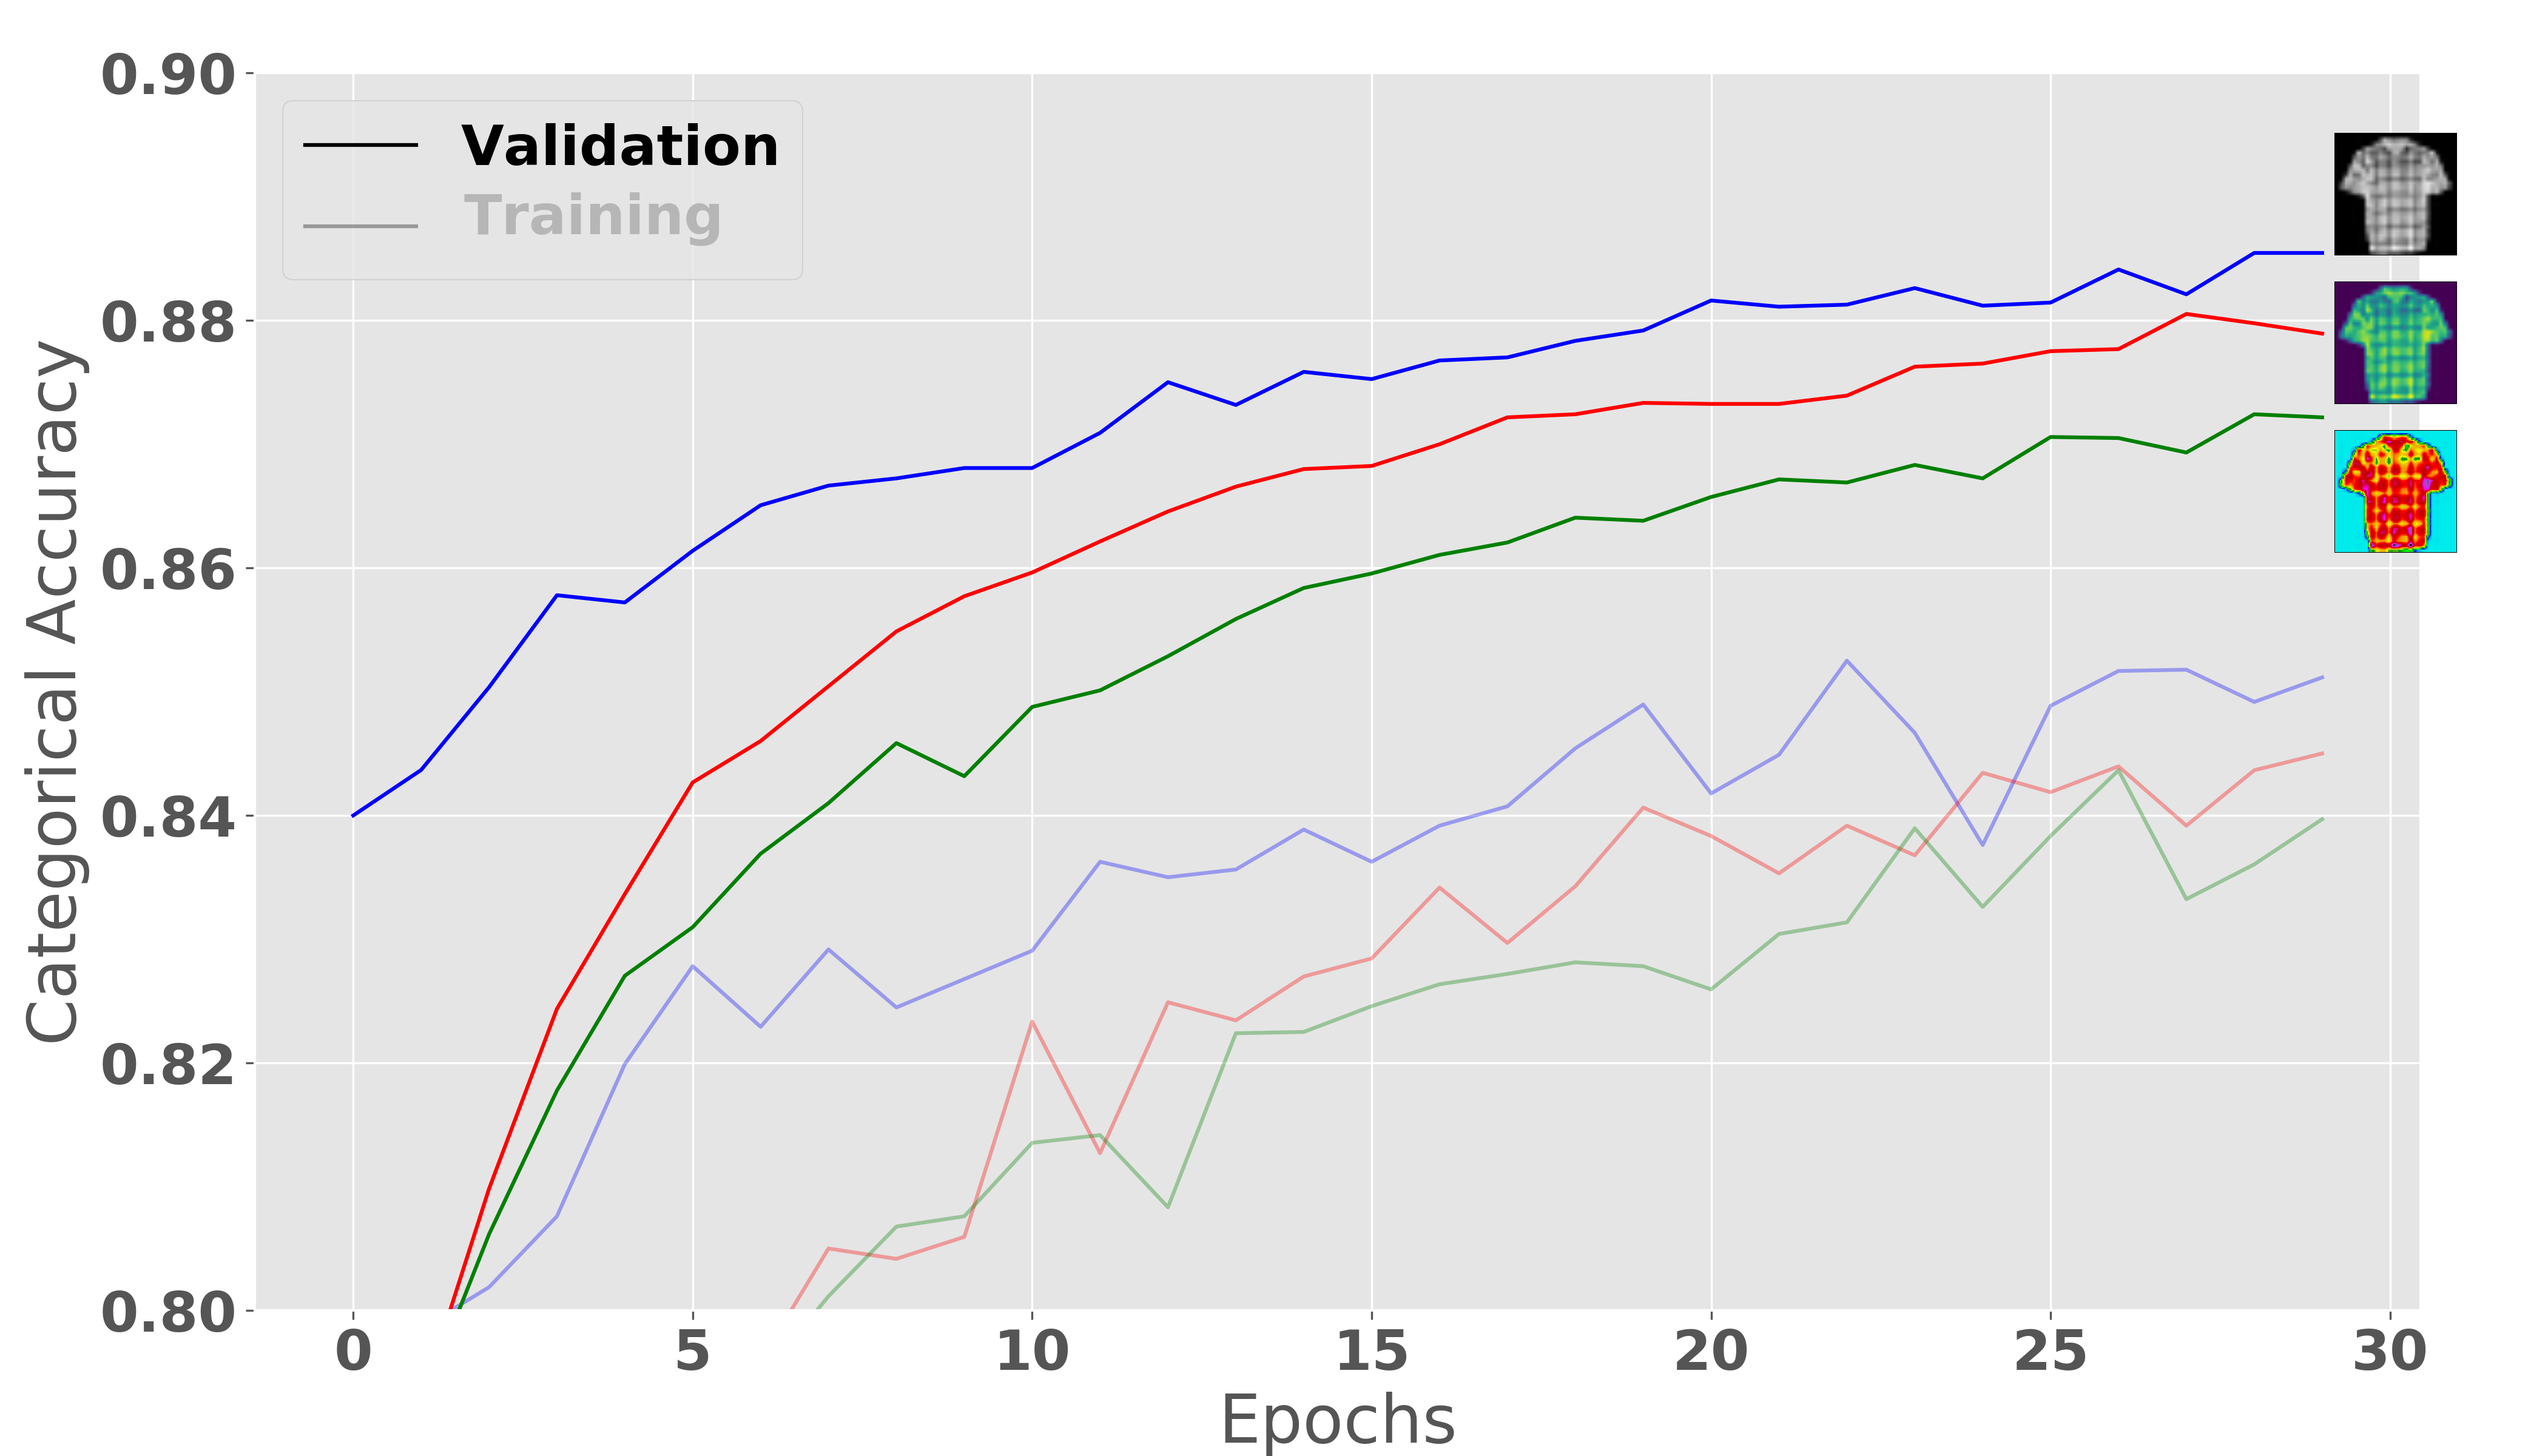
\includegraphics[width=\textwidth]{./thesis_code/plots/train-val-acc_colormaps.png}
	\caption{First 30 epochs in training deep learning model, with input image representations derived from three colormaps, black \& white, viridis, and NWS Reflectivity}
	\label{fig:classifying_colormaps-short-training}
\end{figure}

As before, we see that validation accuracy is higher than training accuracy, while validation loss is lower than training loss, as can be seen when data augmentation is used in training.
This plot shows better results for the data in its original format, with each input channel corresponding to the same intensity values, which renders as a black \& white image.
The viridis colormapped data shows the next best results, followed by the NWS Reflectivity data.
However, it is important to note that at this point in training, each validation accuracy continues to rise.
As such, we should examine the results following a longer period of training, to find where each network learns as much as it can, with respect to classifying new data.

\subsection{Fine Tuning}
\label{ssec:classifying_finetuning}
% Fine tuning experiment to examine validity of this method in classifying data

As demonstrated in Figure \ref{fig:classifying_colormaps-short-training}, the network is able to learn data from each colormap and produce satisfactory validation accuracy results even after 30 epochs of training.
However, it is also apparent that longer training time will continue to increase the learning in the model, as none of the validation accuracy plots have reached a horizontal asymptote.
As such, we can continue training in the model for more epochs to see if the loss and accuracy continues to improve.
To assist in training, we monitor the validation loss, and if 10 epochs of training have passed without an improvement, the learning rate is reduced by a factor of 5.
The motivation for this is that each gradient step after each batch loss is computer is unable to further approach the local minima in the convex region of the multi-dimensional loss function, but that if the learning rate is lowered, gradient steps will be decreased, allowing further training.

Additionally, we employ a technique called \textit{fine tuning}, whereby after a set number of training epochs has reached, all layers in the convolutional base are unfrozen and the entire model is trained for a further number of set epochs.
The idea is that the features extracted in the convolutional base, as trained upon the natural images in ImageNet, are not as accurate on the target task as they could be, and so we must allow the weights in the base model to adapt to this target dataset through more training.
In order to not lose the insights learned when training the top model, however, we set the learning rate to a lower value, so that each gradient step does not drastically change the makeup of a framework that is already working well.

Other authors have attempted to find not only working methods for training such architectures, but to also find optimized versions.
In fact, this process is at the core of \textit{transfer learning}, which again, is the process by which a model is trained deeply and carefully on a source dataset, but is then adapted to a new target task.
Two works stand out from early in the development in this field: \cite{yosinski2014transferable}, which trained AlexNet \cite{krizhevsky2012imagenet} on a few different source tasks and tested on different target tasks; and \cite{oquab2014learning}, which was also based on AlexNet but replaced the final layer with two custom designed layers, making a top classifier to perform object detection on a different (but still natural image) dataset.
The latter stresses the importance of adding layers to assist the network learning to generalize to the new task, while the former illustrates that fine tuning as described above actually led to better results on a target dataset trained from source data, than a network simply trained on the target task in the first place.

The result of this is that we can implement these same concepts using larger networks, and expect to see good results.
To test this hypothesis, we employ the following strategy for each of the three datasets:

\begin{enumerate}
	\item Initialize weights in top classifier, freeze weights in convolutional base (VGG16)
	\item Compile model with adaptive learning rate technique Adam, initial learning rate = $1 x 10^{-4}$
	\item Begin training, 300 batches of size 32 original and augmented images per epoch, for 100 epochs
		\item If a validation set loss plateau is reached, reduce learning rate by factor of 5 and continue training
	\item After 100 epochs: 
		\item Unfreeze all layers in convolutional base
		\item Reset Adam learning rate to $1 x 10^{-5}$ 
		\item Continue training as above
	\item Stop training after a further 100 epochs (total 200)
\end{enumerate}

The goal of this experiment is in part to fundamentally understand that maximum learning capabilities of the end-to-end convolutional neural network model with respect to the various colormapped input datasets.
The results are shown in Figure \ref{fig:classifying_longtraining_finetuning} below.

\begin{figure}[ht]
	\centering
	\begin{subfigure}[b]{\textwidth}
		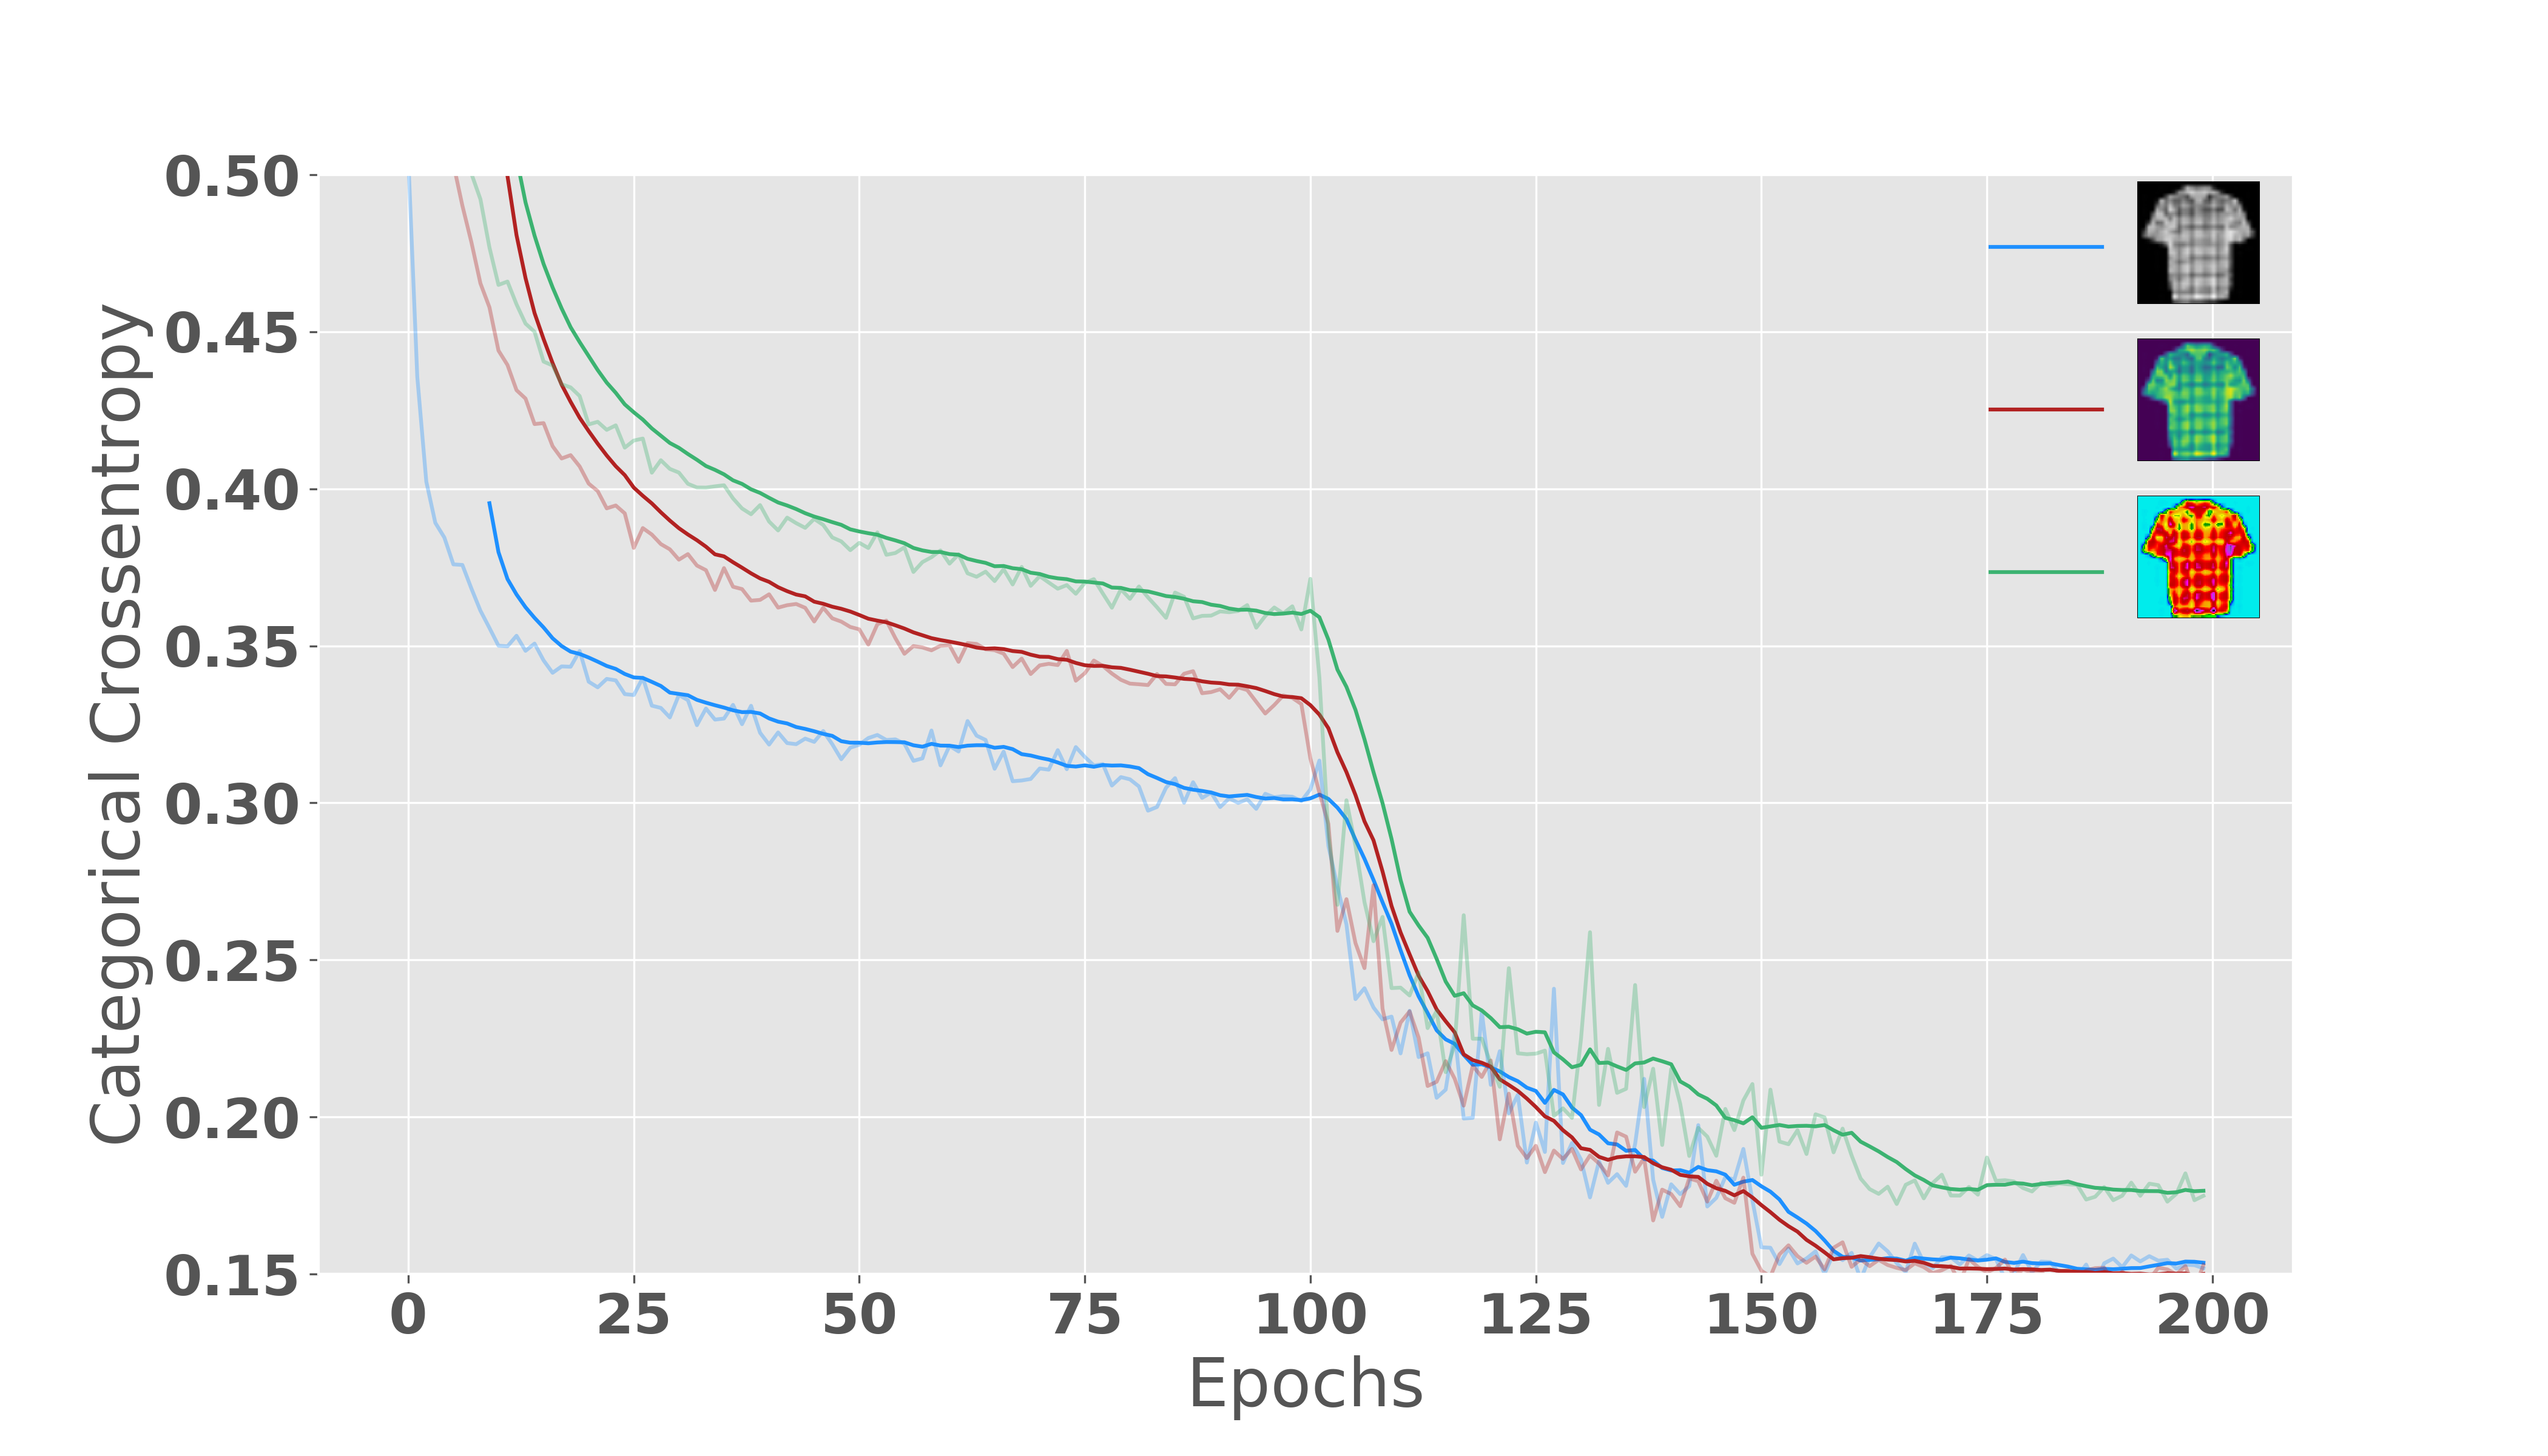
\includegraphics[width=\textwidth]{./thesis_code/plots/20190425_200epoch_finetuning_mnistfashion_loss.png}
		\caption{Loss}
		\label{fig:classifying_longtraining_finetuning_loss}
	\end{subfigure}
	\begin{subfigure}[b]{\textwidth}
		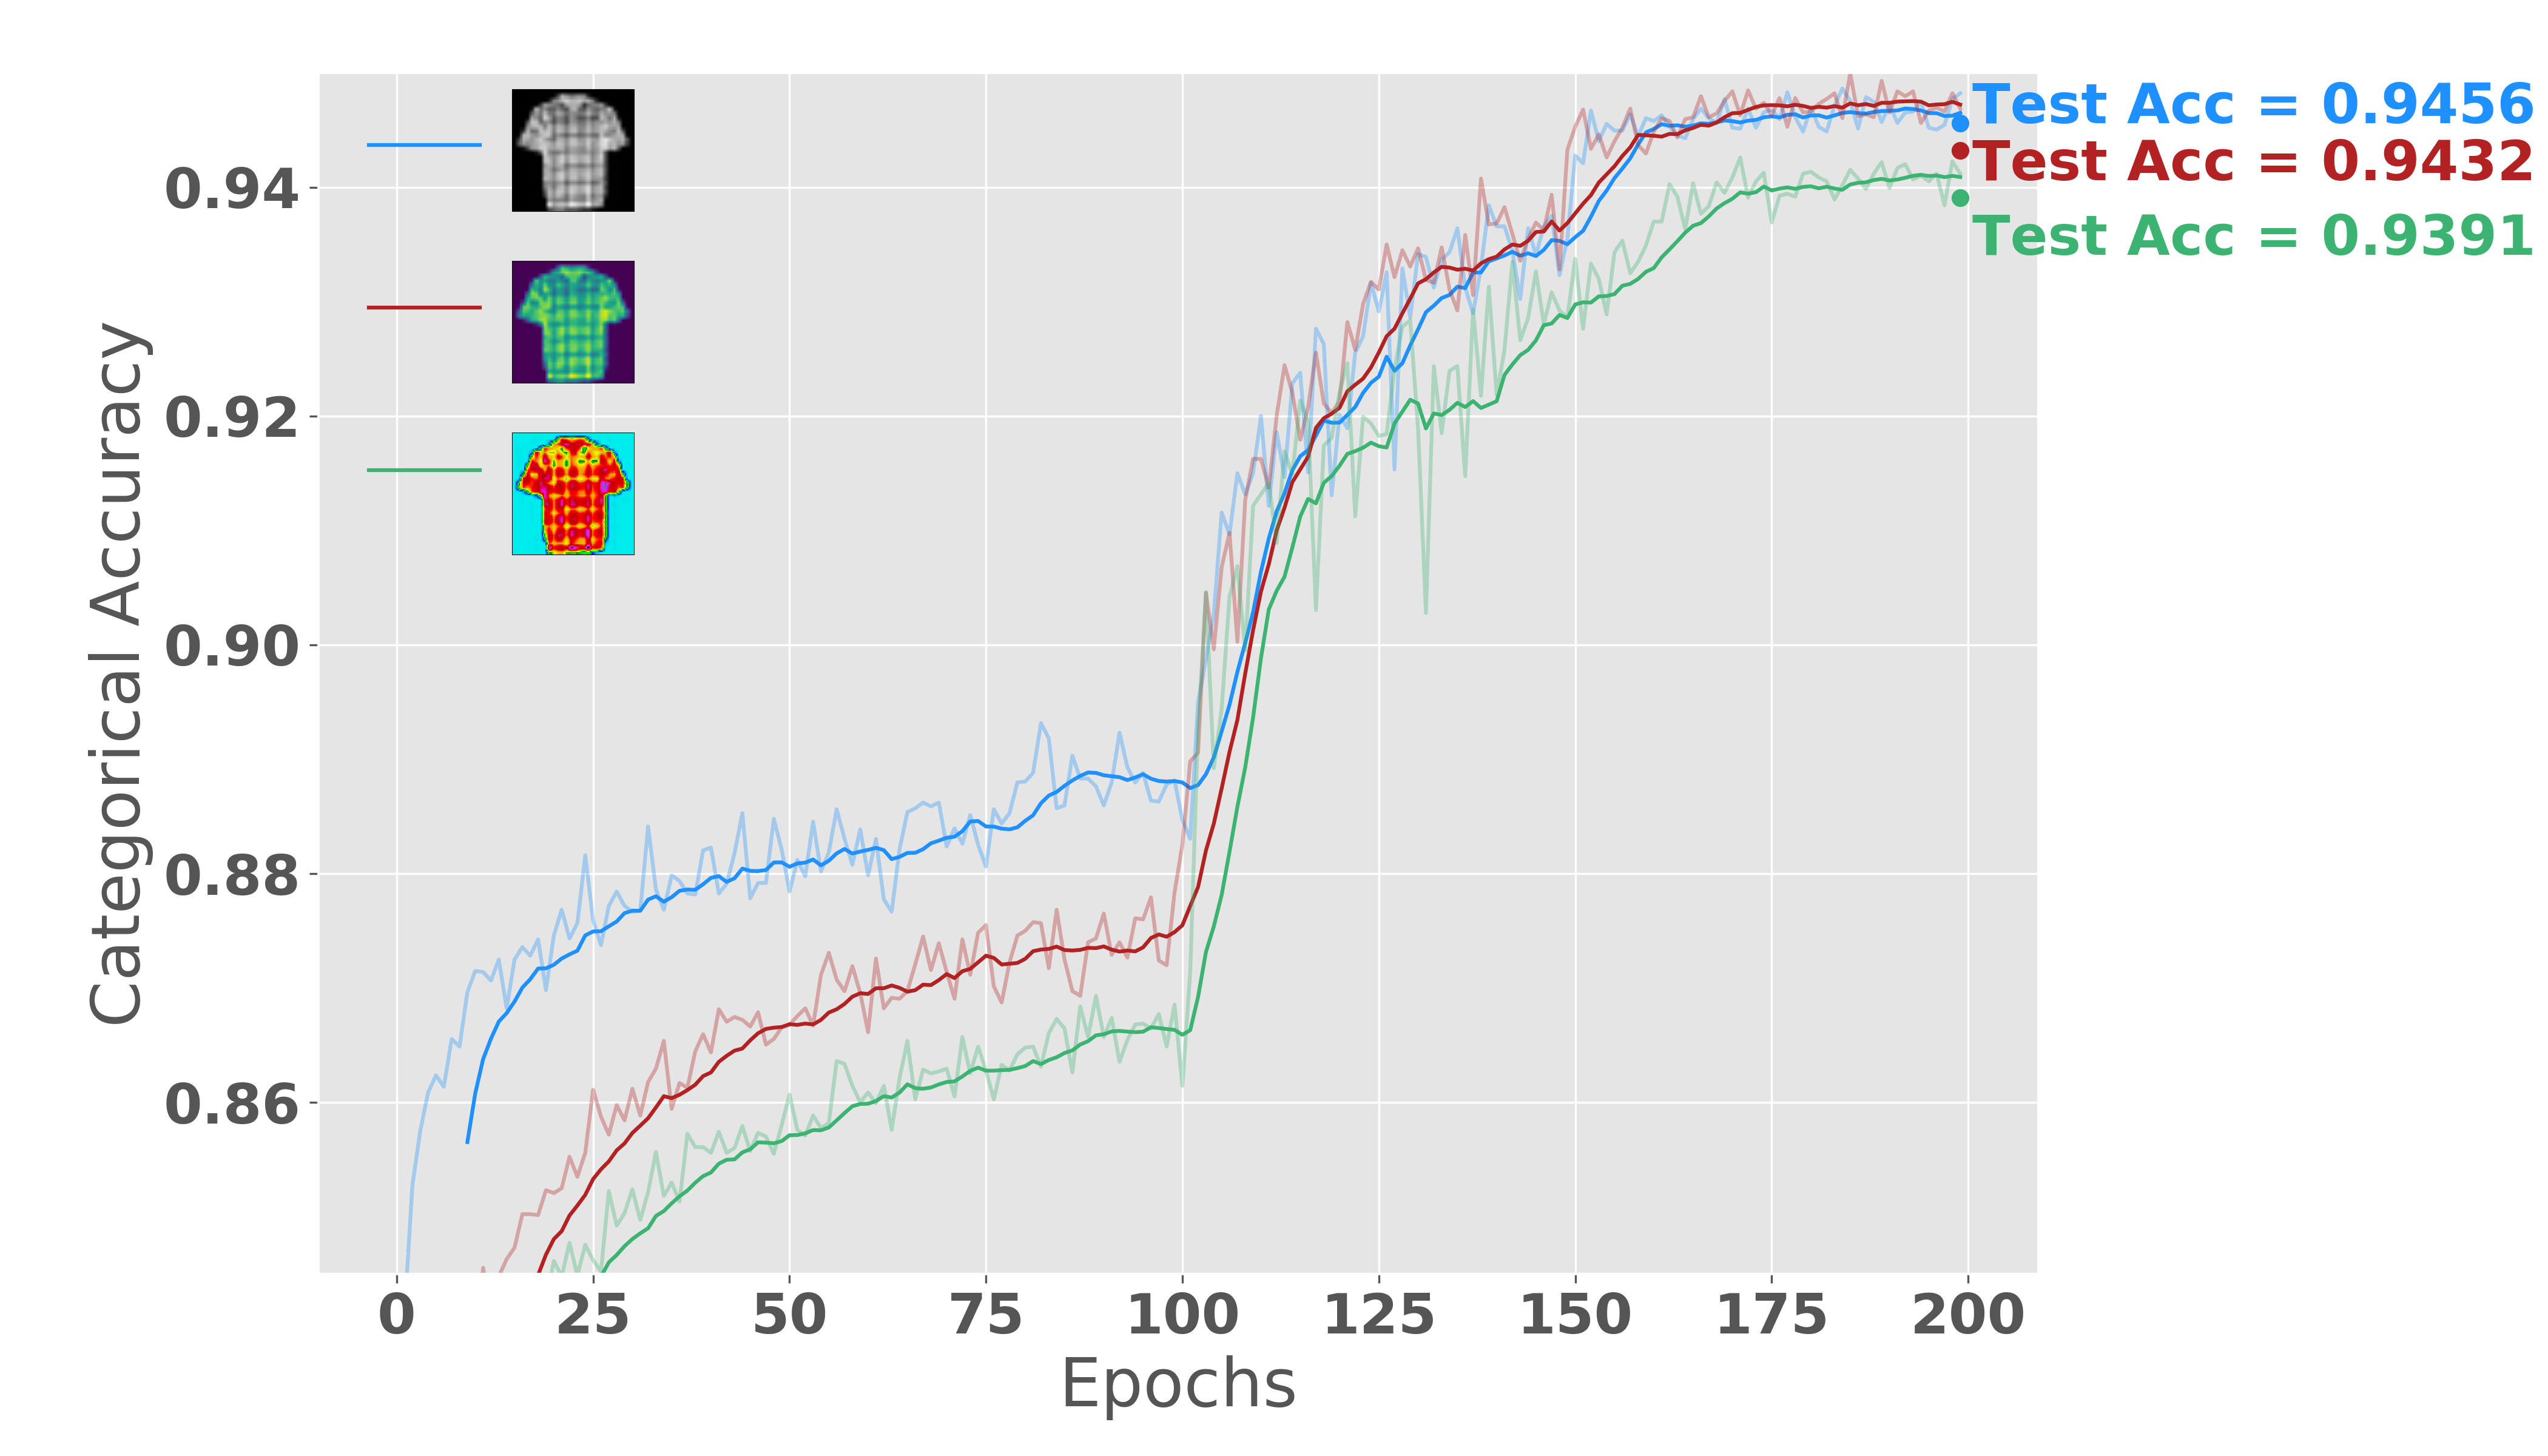
\includegraphics[width=\textwidth]{./thesis_code/plots/20190425_200epoch_finetuning_mnistfashion.png}
		\caption{Accuracy, with final test set accuracy as well}
		\label{fig:classifying_longtraining_finetuning_acc}
	\end{subfigure}
	\caption{Fully training \& fine tuning the VGG16 + top model classifier network on each dataset respectively, and computing learning characteristics. Interestingly, the NWS Reflectivity colormapped data works well, but not as well as both the original dataset, and the viridis colormapped data.}
	\label{fig:classifying_longtraining_finetuning}
\end{figure}

We would expect that the original data has the best results, followed by the colormapped sets, which artificially introduce color mappings to aid human viewing.
Additionally, we expect the NWS Reflectivity to suffer further deleterious effects due to its lower resolution binned color scale, which introduces artificial textures not present in the raw intensity data.
In fact, this is the case, though there are some interesting results to examine.
First, the perceptually uniform colormap, viridis, has nearly the same loss and accuracy curves in the fine tuning phase of training, as well as a similar test set accuracy.
This perhaps may indicate a utility in using perceptually uniform colormaps for not only human visualization but in machine learning settings as well.
Second, while the training characterization suffers when using the NWS Reflectivity colormap, the validation and test set accuracies are still quite good.
For the record, the best test set accuracy on the MNIST-Fashion dataset, using VGG16 as
convolutional base, is 0.935\footnote{\url{https://github.com/zalandoresearch/fashion-mnist}} as of this writing, which all three datasets surpass in this experiment.

The major takeaway here is that colormapped intensity data can provide a useful and satisfactory dataset for transfer learning.
We can have some confidence now, that the model will be able to learn and classify when considering radar data, many variables of which represent intensity values and which are often visualized in colormapped form.
This is particularly useful in the case of the CASA DFW data, which is stored not only in NetCDF form for the raw data, but also has pregenerated radar moments for each scan to assist in human viewing of historical data.
The experiments regarding this data, as well as its usage in classifying precipitation regimes, will be detailed in the next section.

\section{Classifying Reflectivity - CASA DFW}
\label{sec:classifying_zhcasa}

% Hand labeling data from Midlothian, separated into two classes, one for each precipitation regime, 
Data was hand-labeled by the author into one of three classes:

\begin{itemize}
	\item Stratiform Precipitation
	\item Convective Precipitation
	\item Unclassified
\end{itemize}

The first two were labeled when the conditions in Chapter \ref{sec:meteorology} were met for each case.
The third category is considered to be "everything else," for now.
Once these categories were populated, the model described above was trained using the reflectivity pre-generated images as inputs.
The data was split into a training and testing set, where each were about 3 same size, and the testing set was populated with data from completely different days than in training.
When training, the data was further split into two sets, where 90\% of the training set was actually input to the model, and the remaining 10\% was used for computing validation characteristics during training.
It was by monitoring the validation loss and categorical accuracy that we were able to employ an early stopping condition in training, in order to avoid overfitting.
Due to the small size of the dataset, this occurred after only 15 epochs of training.

We must detail a few success metrics here in order to compare the results of this experiment to similar ones described in Chapter \ref{sec:meteorology}.
There are five metrics listed in \cite{anagnostou2004convective}, which we formulate here and compare to the results observed in the present experiment.

Probability of detection (POD) is given by:

\begin{equation}
\mathrm{POD} = \frac{n_{true positive}}{n_{true positive} + n_{false negative}}
\end{equation}

False alarm rate (FAR) is given by:

\begin{equation}
\mathrm{FAR} = \frac{n_{false positive}}{n_{true positive} + n_{false positive}}
\end{equation}

Cumulative success index (CSI) is given by:

\begin{equation}
\mathrm{CSI} = \left[\left(\mathrm{POD}\right)^{-1}+(1-\mathrm{FAR})^(-1)-1\right]^{-1}
\end{equation}

The results from this experiment are detailed in Table \ref{table:classifying_zh_comparison} below. 
The two final parameters from the original paper\cite{anagnostou2004convective} are omitted as they relate to pixels, not only precipitation regime.
Furthermore, the deep neural network presented here (DNN) was trained on a third class to be able to ignore images that were unrelated to stratiform or convective precipitation, which was not performed by the other methods.
As such, we add a third entry to the table below.

\begin{table}
	\begin{tabular}{l l r r r }
		Algorithm & Rain Type & POD & FAR & CSI \\
		\hline
		NN\cite{anagnostou2004convective} & Stratiform & 0.97 & 0.07 & 0.90  \\
		   & Convective & 0.52 & 0.29 & 0.43  \\
		SHY95\cite{steiner1995climatological} & Stratiform & 0.85 & 0.05 & 0.81  \\
		      & Convective & 0.72 & 0.59 & 0.36  \\
		BL00\cite{biggerstaff2000improved} & Stratiform & 0.84 & 0.04 & 0.80  \\
		     & Convective & 0.74 & 0.58 & 0.36 \\
		SHYM\cite{anagnostou2004convective} & Stratiform & 0.89 & 0.05 & 0.85  \\
		     & Convective & 0.69 & 0.51 & 0.40 \\
		\hline
		DNN & Stratiform & 1.00 & 0.00 & 1.00 \\
		    & Convective & 0.99 & 0.04 & 0.96 \\
		DNN & \textbf{Overall} & \textbf{0.976} & \textbf{0.012} & \textbf{0.965} \\
	\end{tabular}
	\caption{Statistics for various algorithms in the literature in calculating stratiform and convective precipitation regimes. The algorithm presented in this research is denoted by DNN, and includes a third class to model all other cases. As such, a row is reported illustrating the overall classification rates, and is bolded to emphasize this.}
	\label{table:classifying_zh_comparison}
\end{table}

\subsection{Data Discovery}
\label{ssec:classifying_discovery}

Deploying the model on CASA DFW servers as a way to identify candidate scans for enlarging precipitation regime dataset, and using iterative, semi-human-supervised process to expand dataset.
Given the complicated nature and lack of conviction regarding directory structural conventions, the CASA DFW servers are particularly challenging to parse.
However, this is a data engineering problem.

As a substitute, several directories were backed up locally to allow deployment of the model and general testing to occur.
The trained model was deployed on two months of data: June 2018 and September 2018. 
For June, convective precipitation was identified, while no stratiform scans were selected.
This is perhaps to be expected, given the warmth in the Dallas-Fort Worth area in the peak summer months, and a higher likelihood of convective activity.
Some sample scans identified are shown below.

\begin{figure}[ht]
	\centering
	\begin{subfigure}[b]{0.45\textwidth}
		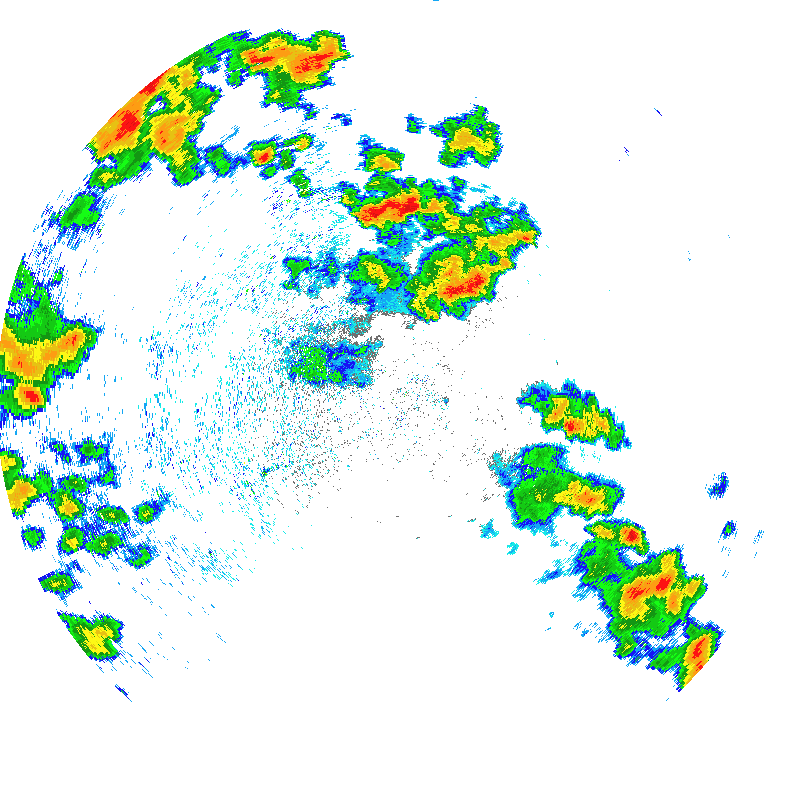
\includegraphics[width=\textwidth]{./thesis_code/plots/midlothian-tx-20180604-115830-ref.png}
		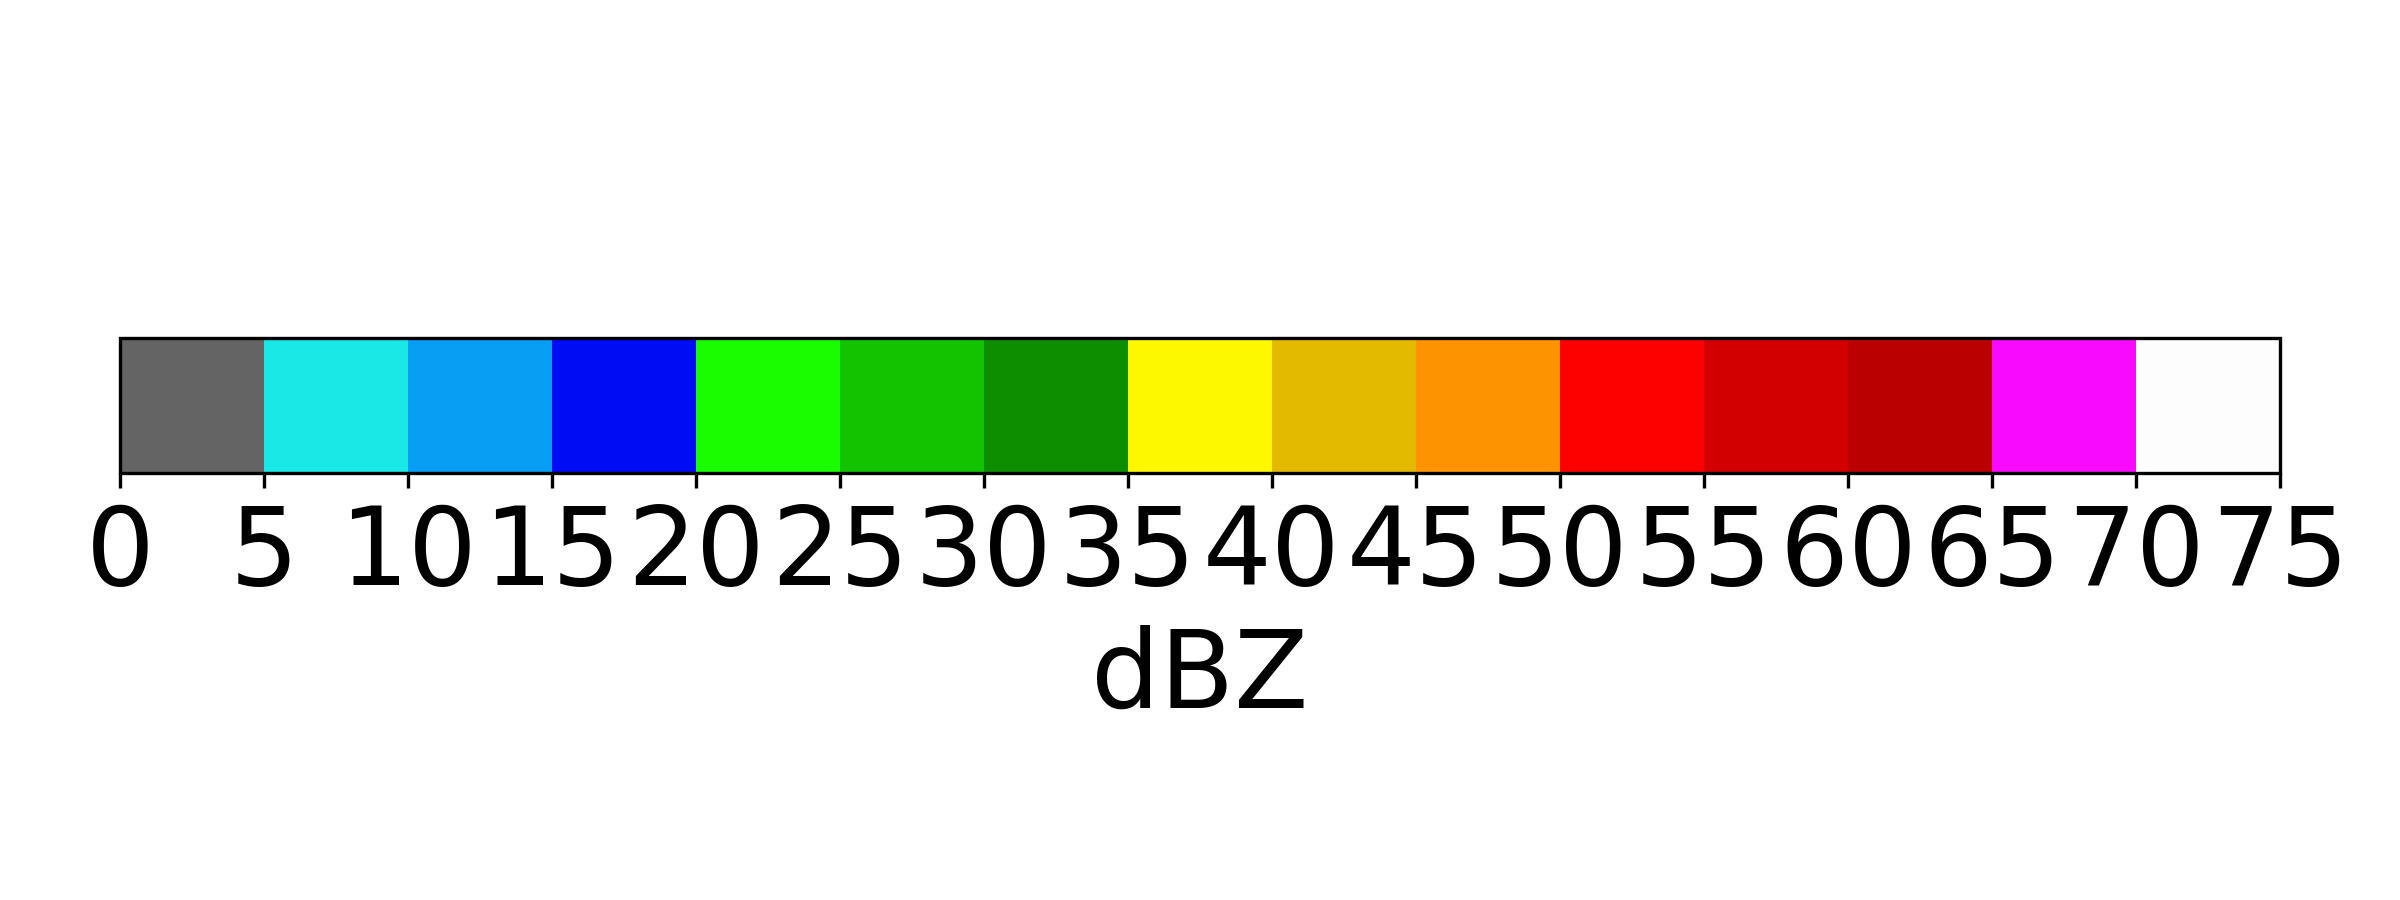
\includegraphics[width=\textwidth]{./thesis_code/plots/dfw_colormap.png}
		\caption{20180604}
		\label{fig:classifying_datadiscovery_ex1}
	\end{subfigure}
	\begin{subfigure}[b]{0.45\textwidth}
		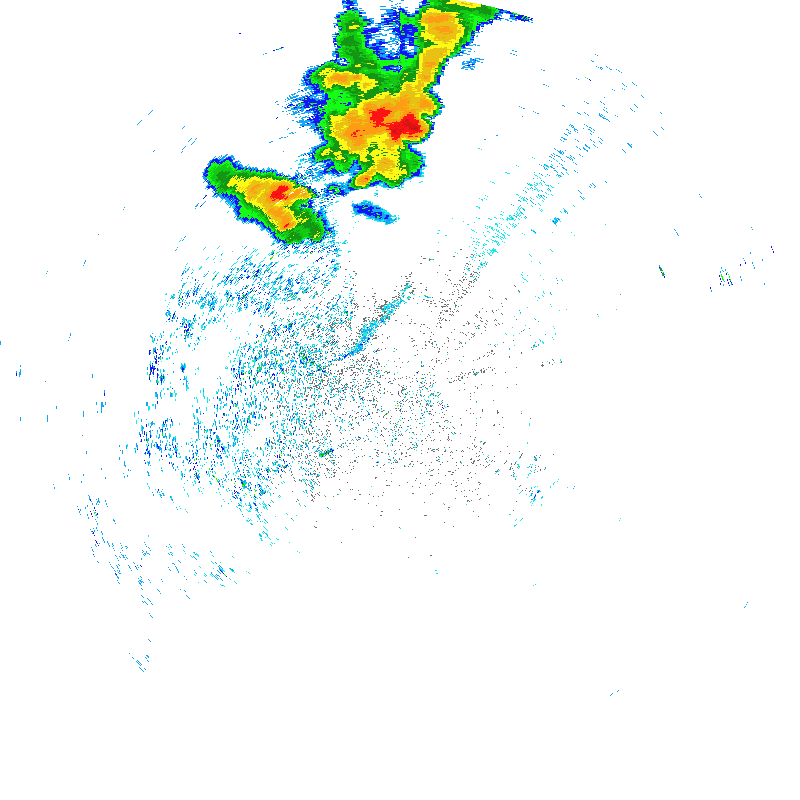
\includegraphics[width=\textwidth]{./thesis_code/plots/midlothian-tx-20180607-233029-ref.png}
		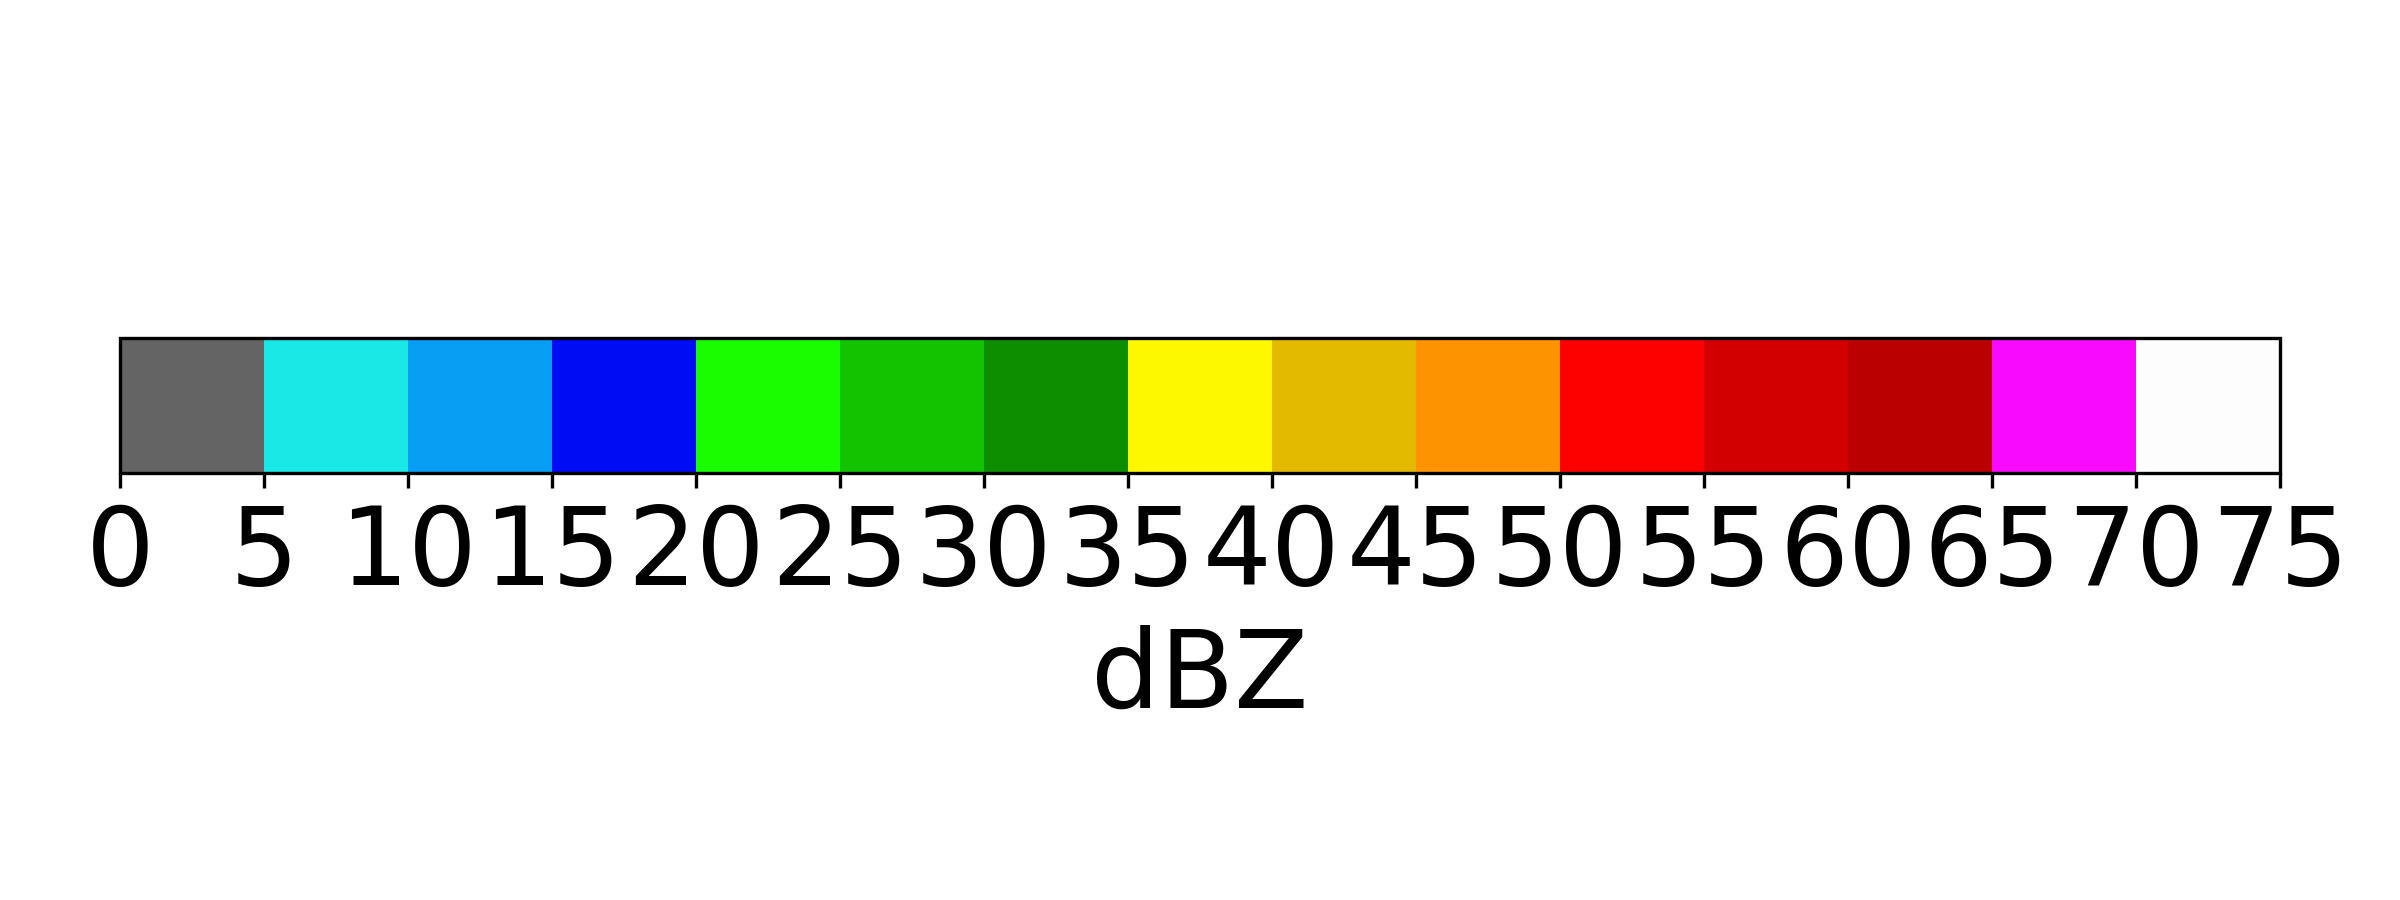
\includegraphics[width=\textwidth]{./thesis_code/plots/dfw_colormap.png}
		\caption{20180607}
		\label{fig:classifying_datadiscovery_ex2}
	\end{subfigure}
	\begin{subfigure}[b]{0.45\textwidth}
		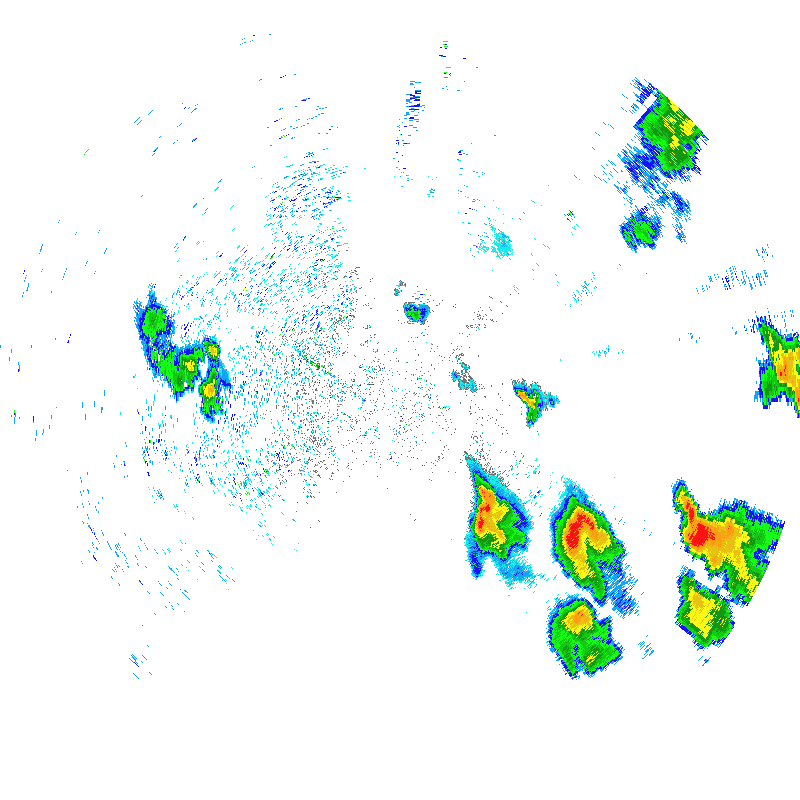
\includegraphics[width=\textwidth]{./thesis_code/plots/midlothian-tx-20180605-104436-ref.png}
		\caption{20180605}
		\label{fig:classifying_datadiscovery_ex3}
	\end{subfigure}
	\begin{subfigure}[b]{0.45\textwidth}
		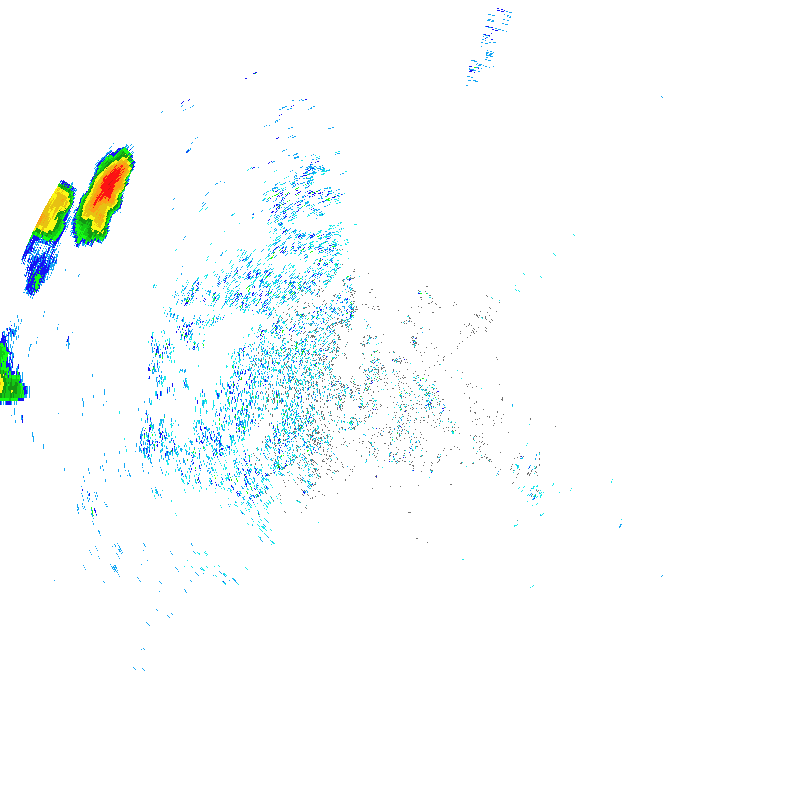
\includegraphics[width=\textwidth]{./thesis_code/plots/midlothian-tx-20180624-063650-ref.png}
		\caption{20180624}
		\label{fig:classifying_datadiscovery_ex4}
	\end{subfigure}
	\caption{Example data that was discovered by model and labeled as convective precipitation. These scans were selected randomly from a large dataset from the month of June 2018, at the XMDL radar. Expert human curation is needed, though these four samples certainly represent the expected precipitation regime.}
	\label{fig:classifying_datadiscovery}
\end{figure}

\begin{figure}[ht]
	\centering
	\begin{subfigure}[b]{0.45\textwidth}
		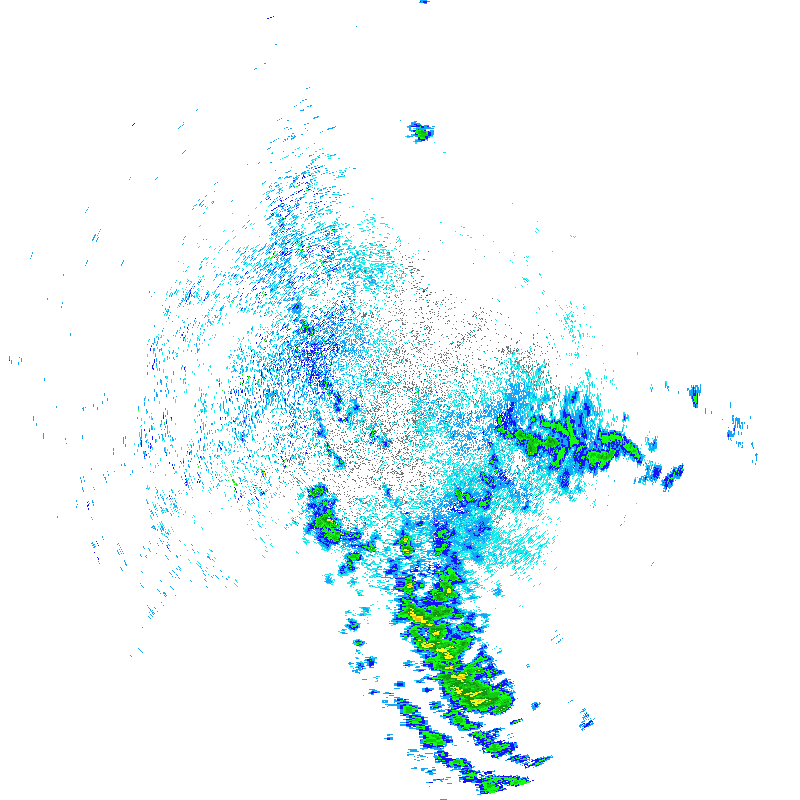
\includegraphics[width=\textwidth]{./thesis_code/plots/midlothian-tx-20180903-063419-ref.png}
		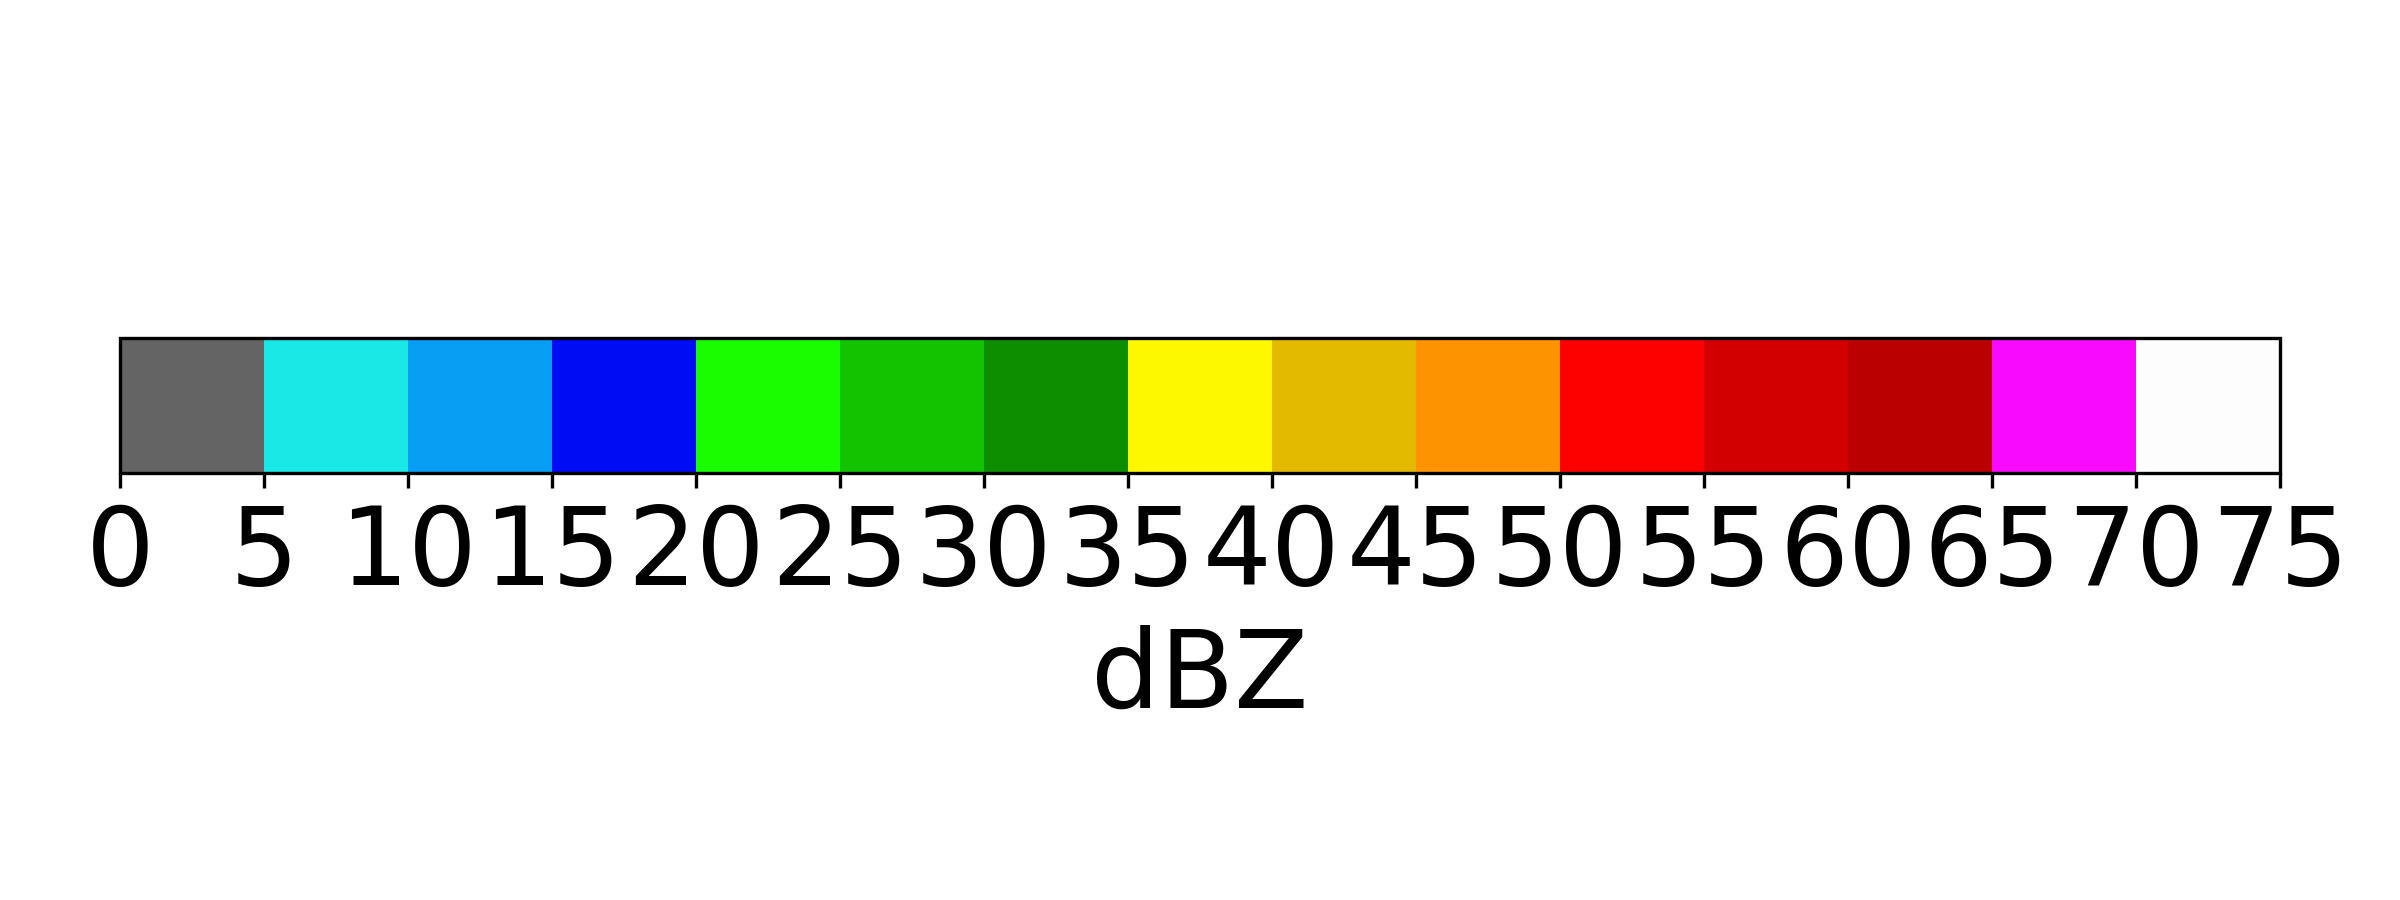
\includegraphics[width=\textwidth]{./thesis_code/plots/dfw_colormap.png}
		\caption{20180903 - Predicted Convective}
		\label{fig:classifying_datadiscovery_ex5}
	\end{subfigure}
	\begin{subfigure}[b]{0.45\textwidth}
		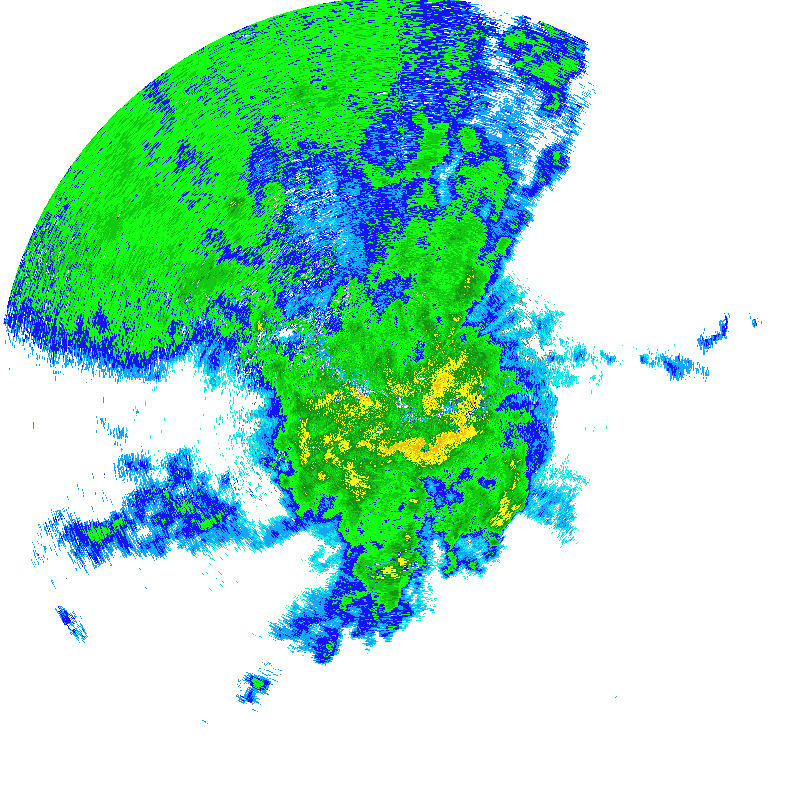
\includegraphics[width=\textwidth]{./thesis_code/plots/midlothian-tx-20180908-173505-ref.png}
		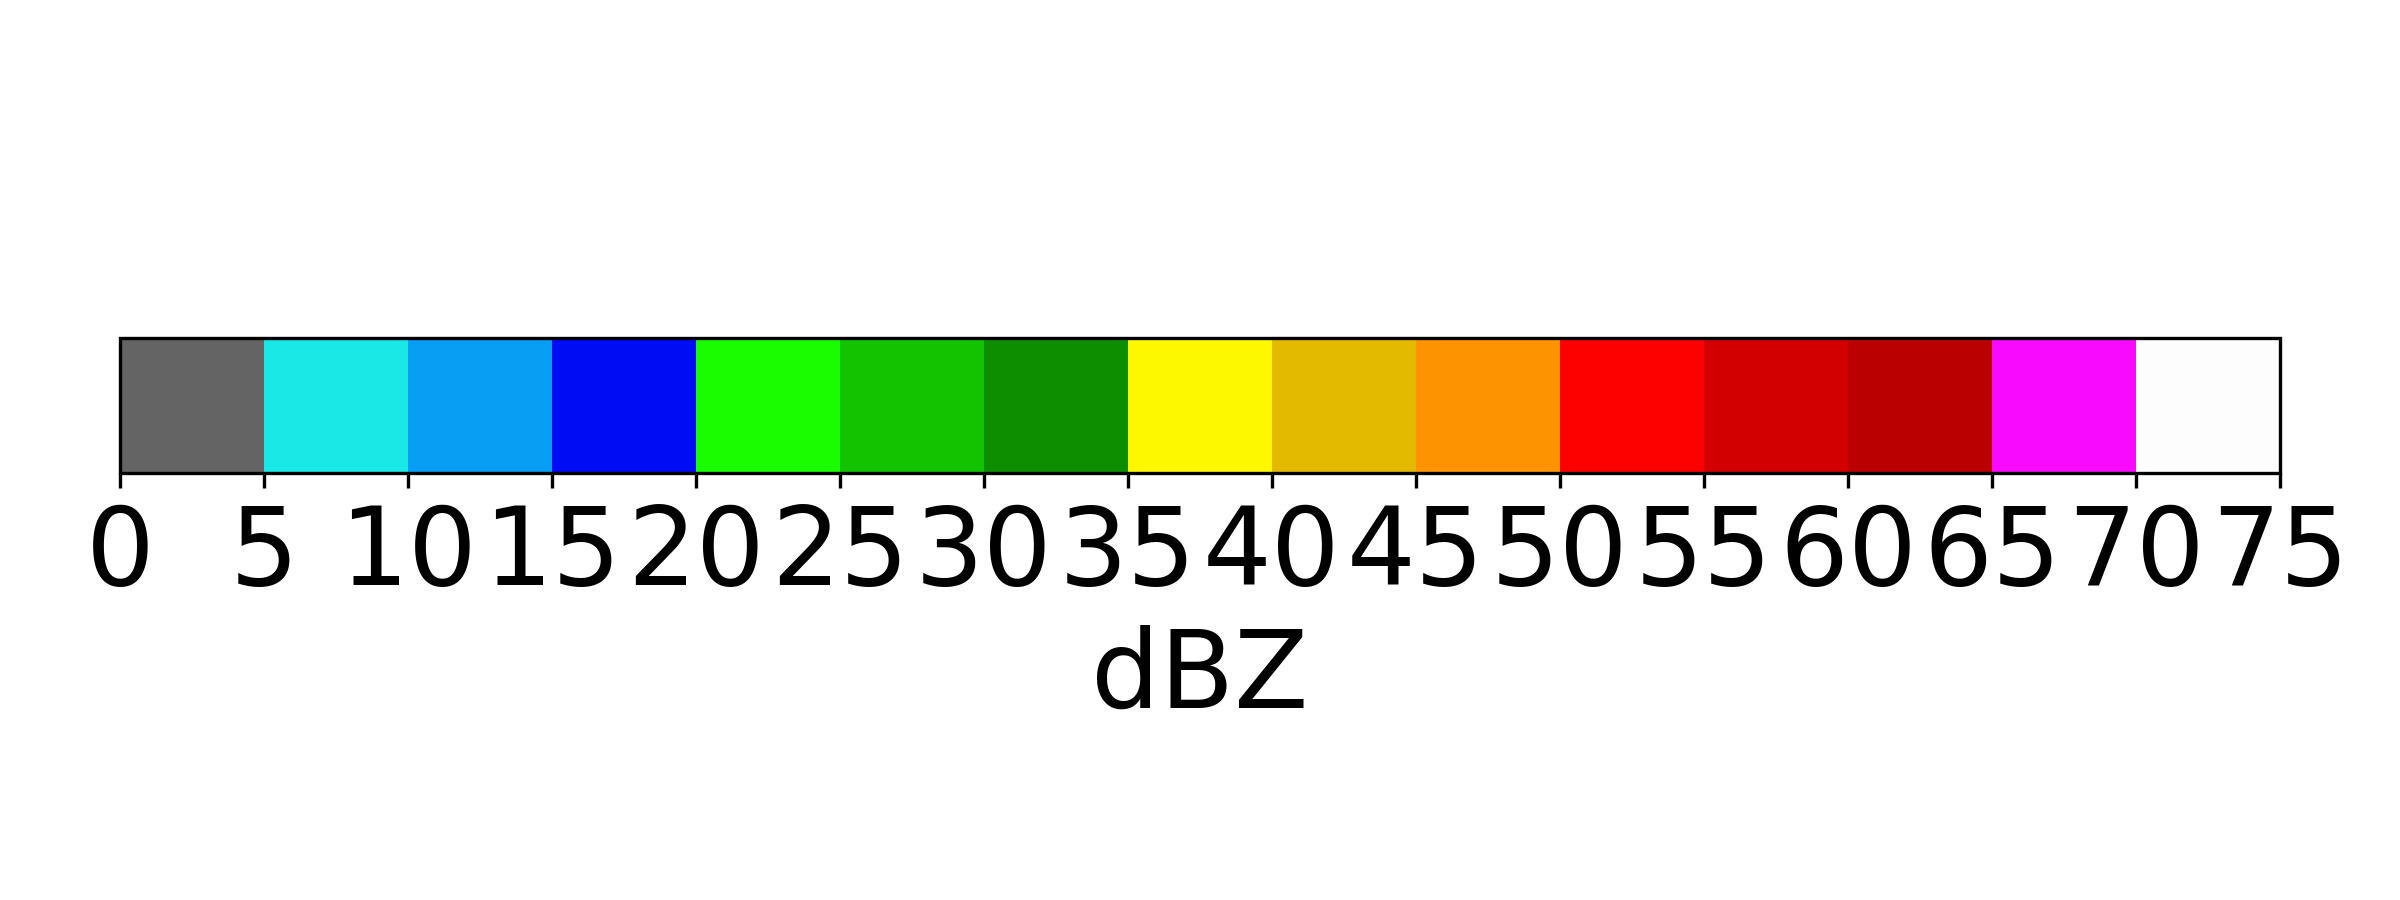
\includegraphics[width=\textwidth]{./thesis_code/plots/dfw_colormap.png}
		\caption{20180908 - Predicted Stratiform}
		\label{fig:classifying_datadiscovery_ex6}
	\end{subfigure}
	\begin{subfigure}[b]{0.45\textwidth}
		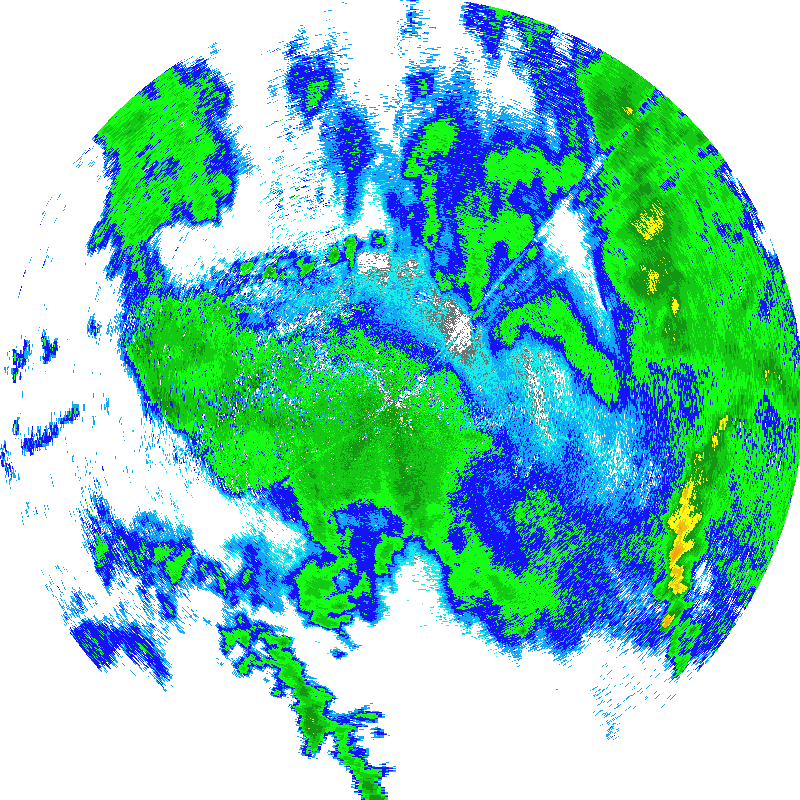
\includegraphics[width=\textwidth]{./thesis_code/plots/midlothian-tx-20180922-105742-ref.png}
		\caption{20180922 - Predicted Stratiform}
		\label{fig:classifying_datadiscovery_ex7}
	\end{subfigure}
	\begin{subfigure}[b]{0.45\textwidth}
		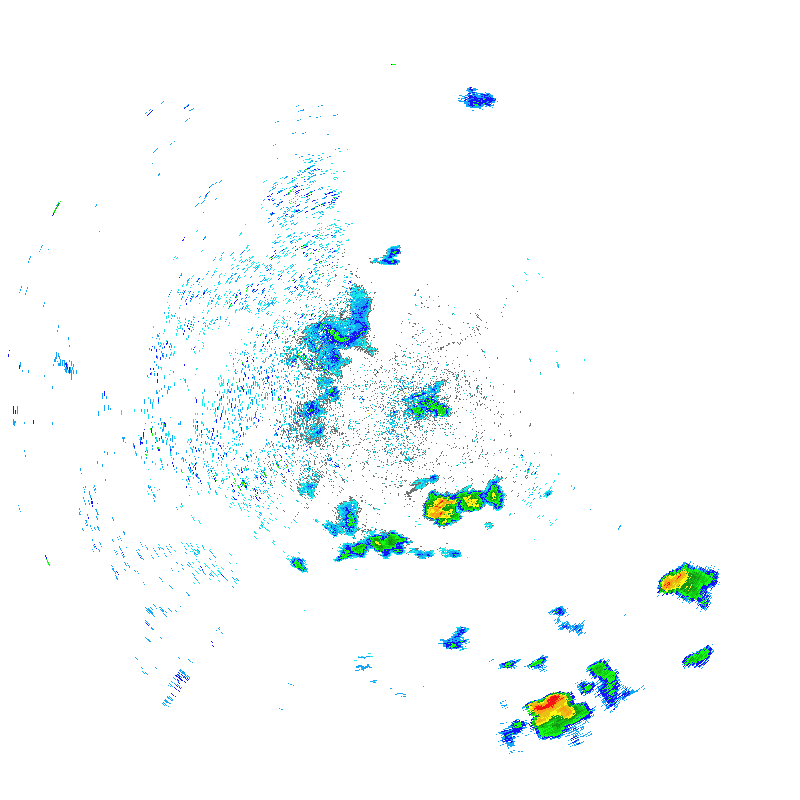
\includegraphics[width=\textwidth]{./thesis_code/plots/midlothian-tx-20180929-202320-ref.png}
		\caption{20180929 - Predicted Stratiform}
		\label{fig:classifying_datadiscovery_ex8}
	\end{subfigure}
	\caption{Example data that was discovered by model. These scans were selected randomly from a large dataset from the month of June 2018, at the XMDL radar. Unlike in Figure \ref{fig:classifying_datadiscovery}, there were more stratiform predictions.}
	\label{fig:classifying_datadiscovery_201809}
\end{figure}

\subsection{CASA - Generated RGB Colormapped Images}
\label{ssec:classifying_casargbdiscovery}

We can generate three-channel pseudo-images where each channel in the image encodes data from different radar variables.
This sort of research has been tested in assisting human visualization and classification before, but it is hypothesized that this could assist a deep learning model in making inferences, especially regarding localized phenomena where radar variable interactions must be considered in order to make correct classifications.
This is an area of proposed research.